\documentclass[preprint,11pt]{elsarticle}

% ====================================================================
% PACKAGES
% ====================================================================
\usepackage{amssymb}
\usepackage{amsmath}
\usepackage{graphicx}
\usepackage{color}
\usepackage{xcolor}
\usepackage{booktabs}
\usepackage[hidelinks]{hyperref}
\usepackage{array}
\usepackage{multirow}
\usepackage{setspace}
\usepackage{siunitx}
\usepackage{cleveref}
\usepackage{placeins}
\usepackage{adjustbox}
\usepackage{etoolbox}
\usepackage{lineno}
\linenumbers
\AtBeginEnvironment{thebibliography}{\footnotesize\setlength{\itemsep}{0pt}\setlength{\parsep}{0pt}}
\setlength{\textfloatsep}{6pt plus 2pt minus 2pt}
\setlength{\floatsep}{6pt plus 2pt minus 2pt}
\setlength{\intextsep}{6pt plus 2pt minus 2pt}
\renewcommand{\topfraction}{0.9}
\renewcommand{\bottomfraction}{0.8}
\renewcommand{\textfraction}{0.1}
\renewcommand{\floatpagefraction}{0.8}
\renewcommand{\dblfloatpagefraction}{0.7}
\setlength{\dblfloatsep}{8pt plus 2pt minus 2pt}
\setlength{\dbltextfloatsep}{8pt plus 2pt minus 2pt}
\emergencystretch=2em
\widowpenalty=10000
\clubpenalty=10000
\renewcommand{\dbltopfraction}{0.9}

\graphicspath{{Figures/}}

% Ragged-right fixed-width column, so wrapped table cells do not stretch
\newcolumntype{L}[1]{>{\raggedright\arraybackslash}p{#1}}

\journal{Chemical Engineering Journal}

\begin{document}

\begin{frontmatter}

% ----------------------------------------------------------------
% TITLE
% ----------------------------------------------------------------
\title{Polyaniline--Silver Metavanadate Nanocomposite Coating for Multi-Gas Detection on a Commercial Metal-Oxide Sensor Platform}

\author[a]{Gayatri Kale}
\author[a]{Apurva Kumar}
\author[b]{Kiran Kokate}
\author[a]{Deepa Nath\corref{cor1}}

\affiliation[a]{organization={Department of Electrical and Electronics Engineering, Dr. Vishwanath Karad MIT World Peace University}, addressline={Survey No. 124, Paud Road, Kothrud}, city={Pune}, state={Maharashtra}, postcode={411038}, country={India}}

\affiliation[b]{organization={Department of Chemistry, School of Science and Environmental Studies, Dr. Vishwanath Karad MIT World Peace University}, addressline={Survey No. 124, Paud Road, Kothrud}, city={Pune}, state={Maharashtra}, postcode={411038}, country={India}}

\cortext[cor1]{Corresponding author. E-mail: deepa.nath@mitwpu.edu.in}

% ----------------------------------------------------------------
% ABSTRACT  (limit: 250 words)
% ----------------------------------------------------------------
\begin{abstract}
We coated a commercial MiCS-4514 gas sensor, which carries two metal-oxide semiconductor (MOX) sensing elements, with a polyaniline (PANI) composite built on a silver metavanadate (AgVO$_3$) precursor, and compared it with an identical uncoated sensor. We made the precursor hydrothermally, polymerised aniline around it in hydrochloric acid and drop-cast the composite in a chitosan-stabilised ink. X-ray diffraction, Fourier-transform infrared spectroscopy and field-emission scanning electron microscopy showed a crystalline silver vanadate precursor with rod-like particles and, in the composite, conducting protonated PANI together with silver chloride formed in the acid step. We exposed both sensors to nitrogen dioxide, ammonia, carbon monoxide and volatile organic compound (VOC) vapour at a nominal 50\% relative humidity and expressed the response with the sensitivity factors defined by the manufacturer. The coated sensor gave a strong, concentration-dependent nitrogen dioxide response above 0.4~ppm, reaching a sensitivity of 44.5 at 1~ppm against 0.93 for the uncoated sensor. Its VOC response exceeded that of the uncoated sensor at every tested concentration, by 11 to 47\%, its ammonia response was indicatively up to 40\% higher between 0.5 and 2~ppm, and its carbon monoxide response was higher up to 7~ppm. The nitrogen dioxide response was at least eight times larger than the response to each of the other gases within the tested windows. The coating thus adds pronounced nitrogen dioxide, VOC and ammonia function to a commercial sensor through a simple, low-cost deposition step.
\end{abstract}

\begin{keyword}
Polyaniline \sep Silver metavanadate \sep Hydrothermal synthesis \sep Gas sensor \sep Nitrogen dioxide \sep Ammonia \sep Chitosan
\end{keyword}

\end{frontmatter}

% ====================================================================
\section{Introduction}
\label{sec:intro}
% ====================================================================

Gas sensing matters for environmental monitoring, industrial safety and indoor air quality, and the spread of Internet-of-Things (IoT) deployments keeps raising the demand for cheap, low-power devices. Two material families dominate the low-cost chemiresistor literature. Metal-oxide semiconductor (MOX) sensors are mature and commercially packaged, but they run hot and discriminate poorly between gases. Conducting polymers work at room temperature, but they drift and lack selectivity on their own. Our work sits at the junction of the two. We coat a polyaniline composite onto a commercial MOX sensor and ask what the coating adds to the part as it is sold.

\subsection{Metal-oxide and polyaniline gas sensors}
\label{sec:lit-mox}
MOX chemiresistors detect gases through changes in a surface depletion layer formed by chemisorbed oxygen. Reducing gases lower the resistance and oxidising gases raise it, and the response is essentially a surface property \cite{fine2010mox}. The usual limits are operation at elevated temperature, cross-sensitivity between reducing species, competition from humidity and baseline drift \cite{fine2010mox,abdullah2022drift}. Recent nanostructured oxides reduce these problems without removing them. Guo et~al.\ \cite{guo2021sno2zno} obtained a response of 336\% to 0.5~parts per million (ppm) of nitrogen dioxide (NO$_2$) at about 20~$^{\circ}$C with ZnO-modified SnO$_2$ nanofibres, and Chu et~al.\ \cite{chu2023ga2o3} reported 1184.6\% to 10~ppm NO$_2$ with Ga$_2$O$_3$ nanorods. Both used custom-built electrodes, and neither addresses discrimination. Room-temperature NO$_2$ sensing is also pursued with two-dimensional MXene layers \cite{radhakrishnan2023mxene}, and ultrathin polymer films laid over oxide sensing layers have been used to tune their selectivity \cite{schroder2023polymerfilms}.

Conducting polymers respond at room temperature, which removes the heater power budget and the thermal-safety limit of MOX devices. Polyaniline (PANI) is the most studied: the monomer is cheap, the synthesis is a simple aqueous oxidative polymerisation, and the conductivity is tuned reversibly by protonation \cite{yang2023panisensors}. Ammonia (NH$_3$) is the textbook analyte. It removes a proton from the emeraldine salt, converts it towards the insulating base and raises the resistance \cite{yang2023panisensors}. Pristine PANI nevertheless has limited selectivity, modest stability, slow recovery and poor batch-to-batch reproducibility, and composites with metal oxides, metal nanoparticles and graphitic carbons are the main route to recover selectivity \cite{masemola2025paniadvances}.

\subsection{PANI--inorganic nanocomposites and chitosan}
\label{sec:lit-composite}
Conducting-polymer/inorganic composites improve on a dense polymer film through three effects acting together: larger surface area and porosity, catalytic or chemical sensitisation by the inorganic phase, and a p--n or p--p junction that modulates conduction more strongly than either component alone \cite{yan2020cpreview}. Zhang et~al.\ \cite{zhang2020panisrge} polymerised PANI in situ on SrGe$_4$O$_9$ nanowires and obtained 20.59\%~ppm$^{-1}$ against 9.82\%~ppm$^{-1}$ for plain PANI over 0.2--10~ppm NH$_3$ at 25~$^{\circ}$C and 60\% relative humidity (RH). This is the closest methodological analogue to our synthesis, because it polymerises aniline around a pre-formed inorganic nanostructure. For NO$_2$, PANI--ZnO thin films have been studied at room temperature \cite{sonker2016panizno}, and Au-decorated ZnO nanofibres coated with PANI act through p--n heterojunctions and Schottky barriers, although at 300~$^{\circ}$C \cite{bonyani2022auzno}. PANI/WS$_2$ has been reported for NH$_3$ \cite{zhao2025paniws2}, and printing of PANI composites has been optimised for sensor fabrication \cite{reiner2022printedpani}.

Silver-containing PANI composites are closer still to our material. Verma and Kumar \cite{verma2024agcupani} reported an 86\% response to 300~ppm NH$_3$ at room temperature for PANI with silver/copper nanoparticles, and Zhou et~al.\ \cite{zhou2024ternary} obtained a response of 3.6 to 500~ppm NH$_3$ with a PANI--copper phthalocyanine--silver ternary film. Al-Mur and Ansari \cite{almur2023agpanimos2} anchored silver on PANI@MoS$_2$ for ammonia and methanol, and Singh et~al.\ \cite{singh2023hcn} followed the same design logic with a non-metallic filler for hydrogen cyanide. Two caveats from this group shape how we read our own results. The reported ammonia concentrations span three orders of magnitude (0.2 to 500~ppm), so a response value only means something when quoted with its concentration, and the response is defined inconsistently, as a percentage sensitivity per ppm, a percentage change or a plain resistance ratio.

Chitosan appears in this literature both as a sensing matrix and as a film-forming binder, and it is the binder in our case. It is not electrochemically inert: chitosan-based films respond to ammonia through the $-$NH$_2$ groups \cite{saeed2024chitosansal}. In a coating formulation it is therefore a variable rather than a neutral binder, and we return to this in \Cref{sec:limitations}.

\subsection{Silver vanadates and $\beta$-AgVO$_3$}
\label{sec:lit-agvo3}
Silver and vanadium form several oxides, and AgVO$_3$ itself crystallises in four polymorphs, of which only the monoclinic $\beta$ phase (space group $Cm$, Joint Committee on Powder Diffraction Standards, JCPDS, card 29-1154) is thermodynamically stable \cite{menezes2019agvo3}. The hydrothermal route gives purer, more crystalline and more reproducible wire-like $\beta$-AgVO$_3$ than precipitation \cite{menezes2019agvo3}. The low-symmetry, multi-reflection diffraction pattern and the one-dimensional morphology are both diagnostic of this phase, and we use them as reference points in \Cref{sec:xrd,sec:fesem}. Gas sensing with silver vanadates is sparse: a single $\beta$-AgVO$_3$ nanowire device for hydrogen sulfide at tens of ppm \cite{mai2010agvo3} and a nanowire breath-humidity sensor \cite{yan2023agvo3breath}. Neither reports CO, NO$_2$ or sub-ppm operation, and neither uses a packaged transducer. The related silver vanadium oxide Ag$_{0.35}$V$_2$O$_5$ has been used for amines \cite{fu2015agv2o5} and, in a TiO$_2$ heterostructure, for ethanol \cite{wang2016tio2agv2o5}.

\subsection{Commercial platform and research gap}
\label{sec:gap}
The MiCS-4514 is a commercial dual-element MOX sensor, with separate reducing (RED) and oxidising (OX) elements on one 5~$\times$~7~$\times$~1.55~mm microelectromechanical system (MEMS) package \cite{sgx2019mics4514}. Its specified ranges are 1--1000~ppm carbon monoxide (CO) on the RED element, 0.05--10~ppm NO$_2$ on the OX element, 1--500~ppm NH$_3$ and 10--500~ppm ethanol, the specified volatile organic compound (VOC) \cite{sgx2019mics4514}. Depositing a secondary layer on its sensing window is an inexpensive way to modify selectivity, provided the coating survives the thermal budget of the sensor. In the literature we reviewed, no study reports a PANI--silver-vanadate composite as a gas-sensing material, and none benchmarks a sensitising overlayer on a packaged MOX sensor against the same uncoated part. Because the transducer is usually bespoke, improvements are referenced to a pristine film of one component rather than to the finished device without its coating. The combination therefore looks relatively unexplored, and we make no priority claim.

\subsection{Objectives}
\label{sec:objectives}
We set out to (1) synthesise the target $\beta$-AgVO$_3$ hydrothermally and coat it in situ with PANI; (2) characterise the precursor and the composite by X-ray diffraction (XRD), field-emission scanning electron microscopy (FESEM) and Fourier-transform infrared (FTIR) spectroscopy and identify the phases present; (3) integrate the composite onto the sensing window as a chitosan-stabilised drop-cast ink and measure the response to CO, NH$_3$, NO$_2$ and VOC vapour against a matched uncoated control; and (4) quantify how the coating changes the response magnitude, selectivity and concentration dependence. \Cref{sec:methods} describes how we made and tested the sensor. \Cref{sec:results} first establishes what we made (\Cref{sec:xrd,sec:fesem,sec:ftir,sec:phase}) and then shows how it changes the response of the sensor (\Cref{sec:gassensing,sec:calibration,sec:ef,sec:selectivity}), followed by a summary, a comparison with the literature and a proposed mechanism (\Cref{sec:summary,sec:comparison,sec:mechanism}). \Cref{sec:limitations,sec:conclusion} state the scope of the work and what we conclude.

% ====================================================================
\section{Materials and Methods}
\label{sec:methods}
% ====================================================================
This section follows the life of one sensor from chemicals to measurement: the materials, the hydrothermal synthesis of the vanadate precursor, the in-situ polymerisation of aniline around it, the fabrication of the coated device, the characterisation of both powders and finally the gas-sensing protocol.


\subsection{Materials}
We used all chemicals as received, without further purification. \Cref{tab:materials} lists the materials with their formulae, suppliers and purities, and their roles are as follows. Ammonium vanadate (NH$_4$VO$_3$) and silver nitrate (AgNO$_3$) were the vanadium and silver precursors for the hydrothermal step, and dilute nitric acid (HNO$_3$) was used only to adjust the pH of the precursor suspension. Aniline (C$_6$H$_5$NH$_2$) was the monomer and ammonium persulfate (APS, (NH$_4$)$_2$S$_2$O$_8$) the oxidant for the in-situ polymerisation, which we carried out in 1~M hydrochloric acid (HCl, diluted from the 37\% stock) as the protonic-acid (doping) medium. Chitosan, a deacetylated polysaccharide with the repeat unit given in \Cref{tab:materials}, was the film-forming binder of the coating ink and was dissolved in aqueous acetic acid (CH$_3$COOH). Absolute ethanol (C$_2$H$_5$OH) was the final washing solvent for the powders and the dispersing solvent of the ink, and distilled water was used for all solutions, dilutions and washing steps. Acetone was used only to clean the sensor window before coating. The substrate was the commercial MiCS-4514 (SGX Sensortech), a dual-element MEMS metal-oxide sensor with separate RED and OX sensing elements.

% Table 1: compiles on its own (pdflatex) and is also \input by main.tex.
\expandafter\ifx\csname documentclass\expandafter\endcsname\csname @notprerr\endcsname\else
\expandafter\ifx\csname documentclass\expandafter\endcsname\csname @twoclasseserror\endcsname\else
\documentclass[11pt]{article}
\usepackage[a4paper,landscape,margin=2cm]{geometry}
\usepackage[T1]{fontenc}
\usepackage[utf8]{inputenc}
\usepackage{times}
\usepackage{amsmath,amssymb}
\usepackage{booktabs,array,multirow,adjustbox,siunitx}
\newcolumntype{L}[1]{>{\raggedright\arraybackslash}p{#1}}

\newcommand{\Cref}[1]{\csname tabref@#1\endcsname}
\renewcommand{\cite}[1]{[\csname tabcite@#1\endcsname]}
\pagestyle{empty}
\setlength{\parindent}{0pt}
\gdef\tabstandalone{1}
\begin{document}
\setcounter{table}{0}
\fi\fi
\begin{table}[!htbp]
\centering
\caption{Chemicals and materials used.}
\label{tab:materials}
\scriptsize
\setlength{\tabcolsep}{3pt}
\begin{adjustbox}{max width=\textwidth,center}
\begin{tabular}{@{}L{4.6cm}L{3.8cm}L{3.4cm}L{4.2cm}@{}}
\toprule
\textbf{Material} & \textbf{Formula} & \textbf{Make} & \textbf{Purity} \\
\midrule
Ammonium vanadate & NH$_4$VO$_3$ & Sigma-Aldrich & $\geq 99\%$ \\
Silver nitrate & AgNO$_3$ & Sigma-Aldrich & $\geq 99.8\%$ \\
Nitric acid & HNO$_3$ & Merck & 68\% \\
Aniline & C$_6$H$_5$NH$_2$ & Sigma-Aldrich & $\geq 99.5\%$ \\
Ammonium persulfate (APS) & (NH$_4$)$_2$S$_2$O$_8$ & Sigma-Aldrich & $\geq 98\%$ \\
Hydrochloric acid & HCl & Merck & 37\% (diluted to 1~M) \\
Chitosan & (C$_6$H$_{11}$NO$_4$)$_n$ & Sigma-Aldrich & 75--85\% deacetylated \\
Acetic acid & CH$_3$COOH & Merck & $\geq 99.8\%$ \\
Ethanol (absolute) & C$_2$H$_5$OH & Merck & $\geq 99.9\%$ \\
Distilled water & H$_2$O & Laboratory & -- \\
Gas sensor & MiCS-4514 & SGX Sensortech & -- \\
\bottomrule
\end{tabular}
\end{adjustbox}
\end{table}
\expandafter\ifx\csname tabstandalone\endcsname\relax\else
\end{document}
\fi


\Cref{fig:synthesis} summarises the whole sequence in five steps. Step 1 combines the vanadium and silver salts at pH 4.5, Step 2 treats the suspension hydrothermally and collects the precursor powder, Step 3 polymerises aniline in cold 1~M HCl in the presence of that powder, Step 4 disperses the composite in a chitosan-stabilised ink, and Step 5 drop-casts the ink onto the sensor, dries it and burns it in. The text under each step in the figure gives the amounts and conditions, and the subsections below give the details. The hydrochloric acid medium of Step~3 matters later, because it is the probable source of the chloride that we find in the composite (\Cref{sec:phase}).

\begin{figure}[!htbp]
\centering
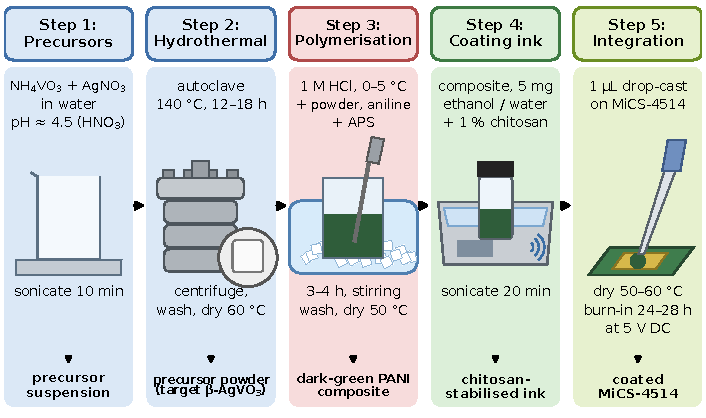
\includegraphics[width=\textwidth]{Figure_1.pdf}
\caption{Synthesis and coating route. Schematic redrawn as vector graphics from a Google Gemini draft.}
\label{fig:synthesis}
\end{figure}

\subsection{Synthesis of the vanadate precursor by the hydrothermal method}
\label{sec:synth-vanadate}
We dissolved NH$_4$VO$_3$ (0.5~g, 4.27~mmol) in 30~mL of distilled water at $\sim$40~$^{\circ}$C and added AgNO$_3$ (0.72~g, 4.24~mmol) in 20~mL of distilled water dropwise over 10~min. The two salts are therefore close to equimolar, as the 1:1 Ag:V ratio of AgVO$_3$ requires. We adjusted the pH to $\sim$4.5 with dilute HNO$_3$, sonicated the suspension for 10~min, transferred it to a Teflon-lined autoclave and heated it at 140~$^{\circ}$C for 12--18~h. After natural cooling we collected the precipitate by centrifugation (6000~rpm, 10~min), washed it three times with distilled water and once with ethanol, and dried it at 60~$^{\circ}$C overnight. The yield was 85--90\%. This step was aimed at $\beta$-AgVO$_3$, and \Cref{sec:results} reports the characterisation of the product.

\subsection{In-situ PANI polymerisation}
\label{sec:synth-pani}
We dispersed the vanadate powder (100~mg) in 40~mL of chilled 1~M HCl (0--5~$^{\circ}$C) and sonicated it for 5~min. After adding aniline (0.925~mL, about 10.2~mmol, taking a density of 1.022~g~mL$^{-1}$) we stirred the dispersion for 10--15~min. APS at an aniline:APS molar ratio of 1:1.25 (about 12.7~mmol, or 2.9~g) was dissolved in distilled water and added dropwise to start the polymerisation, which ran for 3--4~h at 0--5~$^{\circ}$C under continuous stirring. We filtered the product, washed it to neutral pH, gave it a final ethanol rinse and dried it at 50~$^{\circ}$C for 4~h, which gave a dark-green composite powder. The dark-green colour is typical of the protonated, conducting emeraldine-salt form of PANI \cite{yang2023panisensors}.

\subsection{Sensor fabrication}
\label{sec:fabrication}
We prepared a 1\% chitosan solution in 1\% aqueous acetic acid as the binder. The coating ink contained composite powder (5~mg), absolute ethanol (0.5~mL), distilled water (0.5~mL) and chitosan solution (20~$\mu$L), and was sonicated for 20~min. We cleaned the MiCS-4514 sensing window with acetone, let it air-dry, and deposited 1~$\mu$L of ink at the centre of the sensing window with a micropipette. The coated device was oven-dried at 50--60~$^{\circ}$C for 1--2~h, connected to an ESP32 microcontroller board (Espressif Systems), powered at 5~V direct current (DC) and run continuously for 24--28~h to stabilise the baseline resistance before testing (\Cref{fig:setup}). The board supplied the heater network through the manufacturer-specified dropping resistors (82~$\Omega$ for the RED element and 133~$\Omega$ for the OX element) and read the voltage across load resistors (100~k$\Omega$ for the RED element and 220~$\Omega$ for the OX element) to obtain the sensing resistance $R_s$ of each element \cite{sgx2019mics4514}. We coated one sensor and left the other sensor uncoated.

\begin{figure}[!htbp]
\centering
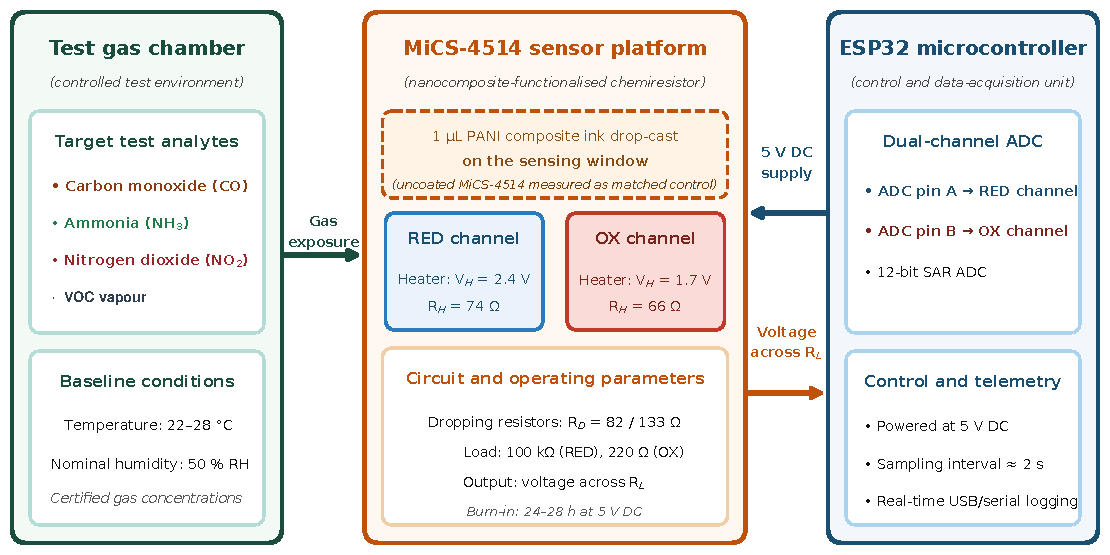
\includegraphics[width=\textwidth]{Figure_2.pdf}
\caption{Experimental setup and read-out chain.}
\label{fig:setup}
\end{figure}

\subsection{Material characterisation}
\label{sec:characterisation}
We recorded powder XRD on a PANalytical Empyrean diffractometer (Cu K$\alpha_1$ = 1.54060~\AA, K$\alpha_2$ = 1.54443~\AA, intensity ratio 0.500; 45~kV, 40~mA) over 2$\theta$ = 5.1--79.9$^{\circ}$ in continuous mode, with a step size of 0.0167$^{\circ}$ (4479 points), 8.255~s per step, a fixed 0.19~mm divergence slit and no monochromator. Both powders were measured as flat samples under identical settings. FESEM was done on a TESCAN CLARA instrument at 15~kV with an Everhart--Thornley detector, a 2.99~nm spot size and a working distance of 9.7--9.8~mm, at magnifications from 1000$\times$ to 75\,000$\times$. FTIR transmittance spectra were recorded on a Shimadzu spectrometer over 400--4500~cm$^{-1}$ at a resolution of 2~cm$^{-1}$, averaging 40 scans with Happ--Genzel apodisation. In the figures and tables we label the hydrothermal precursor AgVO$_3$ and the composite polymerised in 1~M HCl PA-HCl. XRD, FTIR and FESEM were recorded on both powders.

\subsection{Gas-sensing measurements}
\label{sec:gas-methods}
We coated one MiCS-4514 sensor and left a nominally identical second sensor uncoated as the control. Both were connected to an ESP32 board, which biased the RED and OX heater and sensing elements and digitised the voltages across their load resistors (\Cref{fig:setup}). \Cref{fig:setup} reads from left to right. The test gas chamber holds the sensor at controlled temperature and humidity. The MiCS-4514 platform carries the RED and OX channels, each with its heater and load-resistor network. The ESP32 board supplies 5~V DC to the heaters and biases each sensing element at 3.3~V through its load resistor. It reads the voltage across each load resistor through two analogue-to-digital converter (ADC) pins with 11~dB input attenuation and logs the counts over a universal serial bus (USB) link at intervals of $\sim$2~s. The converter is a 12-bit successive-approximation-register (SAR) type. The certified concentration and the chamber temperature were entered into the logger by the operator whenever they changed, and the humidity field was held at the nominal 50\% RH, so that every logged line carries its set-point. Tests were run at a nominal 50\% relative humidity (RH) and at chamber temperatures of 22--28~$^{\circ}$C against certified concentrations of CO (0.5--13~ppm), NH$_3$ (0.01--2~ppm), NO$_2$ (0.05--1~ppm) and VOC vapour (0.01--0.3~ppm). Each gas was run once on the coated sensor and once on the uncoated sensor.

The circuit follows the data sheet \cite{sgx2019mics4514}. The two heaters ran from the 5~V supply (specified 4.9--5.1~V) through series dropping resistors of 82~$\Omega$ for the RED element and 133~$\Omega$ for the OX element (51 + 82~$\Omega$), which give the typical heater voltages of 2.4~V (RED) and 1.7~V (OX), heater resistances of 74 and 66~$\Omega$ at nominal power, heater currents of 32 and 26~mA and heater powers of 76 and 43~mW. These values agree with Ohm's law: $(5-2.4)/82 = 32$~mA and $(5-1.7)/133 = 25$~mA, and $2.4\times 32\approx 77$~mW and $1.7\times 26\approx 44$~mW. The data sheet gives the sensing resistance in air as 100--1500~k$\Omega$ for the RED element and 0.8--20~k$\Omega$ for the OX element, measured at 23~$\pm$~5~$^{\circ}$C and 50~$\pm$~10\% RH for the RED and at $\leq 5$\% RH for the OX element.

Each gas series followed a stepped protocol. After a zero-gas baseline segment we raised the analyte concentration in discrete increments across the tested range, and each level was held for about 6~min. A complete concentration--response curve for one gas therefore comes from a single continuous log lasting roughly 65 to 95~min, in which each step starts from the state left by the previous one.

The ADC count of each element was converted to the sensing resistance with the voltage-divider relation of the read-out,
\begin{equation}
R_{s} \;=\; R_{L}\left(\frac{4095}{\mathrm{ADC}}-1\right),
\label{eq:rs}
\end{equation}
where $R_{L}$ is the load resistance of the element (100~k$\Omega$ for the RED element and 220~$\Omega$ for the OX element) and 4095 is the full-scale count of the 12-bit converter. We took $R_{0}$ as the mean resistance of the clean-air segment at the start of the same run, so that $R_0$ is recomputed for every run and every element and is never carried over from another run. We express the response with the two sensitivity factors that the data sheet uses. It defines $S_{60}=R_{s}(\mathrm{air})/R_{s}(60~\mathrm{ppm~CO})$ for the RED element and $S_R=R_{s}(0.25~\mathrm{ppm~NO_2})/R_{s}(\mathrm{air})$ for the OX element, and we generalise these to
\begin{equation}
S_{\mathrm{RED}} \;=\; \frac{R_{0}}{R_{s}}, \qquad S_{\mathrm{OX}} \;=\; \frac{R_{s}}{R_{0}},
\label{eq:S}
\end{equation}
where $R_s$ is the mean resistance of a concentration step. Both factors equal 1 when the gas has no effect and exceed 1 when the resistance moves in the direction that the element responds to: $S_{\mathrm{RED}}$ when the RED resistance falls, as for CO and VOC vapour, and $S_{\mathrm{OX}}$ when the OX resistance rises, as for NO$_2$ and, in our runs, for NH$_3$. Neither factor is bounded above. We report $S_{\mathrm{RED}}$ for CO and VOC vapour and $S_{\mathrm{OX}}$ for NO$_2$ and NH$_3$.

We described the dependence of $S$ on the concentration $C$ with the empirical power law
\begin{equation}
S \;=\; A\,C^{B},
\label{eq:power}
\end{equation}
where $A$ is the sensitivity at 1~ppm and $B$ an exponent that is below 1 for a saturating response and above 1 for a response that steepens with concentration, or with a second-order polynomial $S = aC^{2}+bC+c$ where the power law did not describe the data. We fitted both by least squares to the step means and judged each fit by its coefficient of determination $R^{2}$ and root-mean-square error (RMSE). To compare the coated and uncoated sensors at the same concentration we used the sensitivity enhancement $E$ and the enhancement factor (EF),
\begin{equation}
E \;=\; \frac{S_{\mathrm{coated}}-S_{\mathrm{uncoated}}}{S_{\mathrm{uncoated}}}\times 100\%, \qquad \mathrm{EF} \;=\; \frac{S_{\mathrm{coated}}}{S_{\mathrm{uncoated}}},
\label{eq:enh}
\end{equation}
which are positive (EF above 1) when the coated sensor responds more strongly and negative (EF below 1) when it responds less.


% ====================================================================
\section{Results and Discussion}
\label{sec:results}
% ====================================================================
We first establish what is on the sensor (\Cref{sec:xrd,sec:fesem,sec:ftir,sec:phase}) and then describe how it changes the response of the sensor (\Cref{sec:gassensing,sec:calibration,sec:ef,sec:selectivity,sec:summary,sec:comparison,sec:mechanism}). This order lets the identity of the material guide the reading of the sensing results.


\subsection{Structural characterisation (XRD)}
\label{sec:xrd}
We start with diffraction, because the phase identity of the inorganic component decides how everything that follows has to be read.


\begin{figure}[!htbp]
\centering
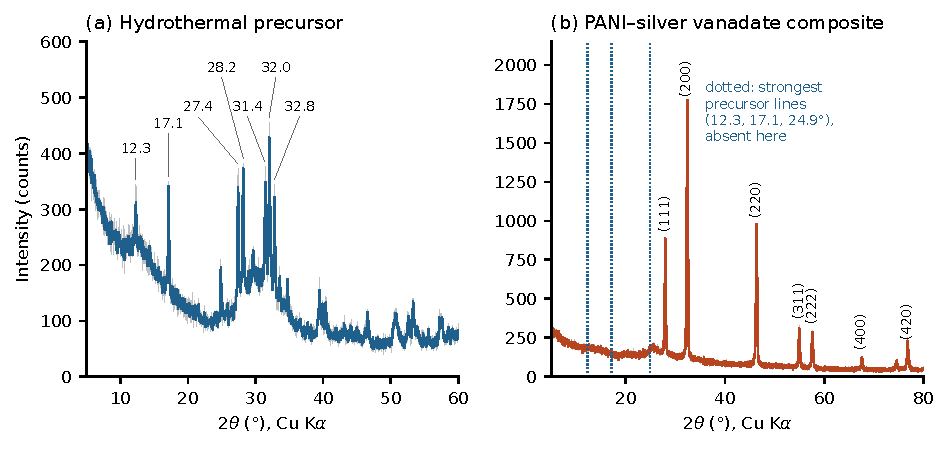
\includegraphics[width=\textwidth]{Figure_3.pdf}
\caption{Powder XRD patterns of (a) the precursor and (b) the composite.}
\label{fig:xrd}
\end{figure}

\Cref{fig:xrd} shows the two diffraction patterns, \Cref{tab:xrdp} lists the reflections of the precursor and \Cref{tab:xrd} those of the composite. We converted peak positions to interplanar spacings with Bragg's law for first-order reflection,
\begin{equation}
2\,d\sin\theta = \lambda,
\label{eq:bragg}
\end{equation}
where $d$ is the interplanar spacing, $\theta$ the Bragg angle and $\lambda = 1.5406$~\AA{} the Cu K$\alpha_1$ wavelength. For a cubic lattice with lattice parameter $a$, the spacing of the $(hkl)$ planes follows
\begin{equation}
\frac{1}{d_{hkl}^{2}} = \frac{h^{2}+k^{2}+l^{2}}{a^{2}},
\label{eq:cubic}
\end{equation}
and we estimated the apparent crystallite size $D$ with the Scherrer equation,
\begin{equation}
D = \frac{K\lambda}{\beta\cos\theta},
\label{eq:scherrer}
\end{equation}
where $K = 0.9$ is the shape factor and $\beta$ the full width at half maximum (FWHM) in radians. We fitted every reflection with a pseudo-Voigt profile for the K$\alpha_1$ and K$\alpha_2$ doublet on a linear background and took $\beta$ from the K$\alpha_1$ component. We made no correction for instrumental broadening, so $D$ is an apparent value and a lower bound. As a consistency check, recomputing $d$ from the tabulated $2\theta$ values with \Cref{eq:bragg} reproduces the listed $d_{\mathrm{obs}}$ to within 0.003~\AA{} (the $2\theta$ values are rounded to 0.01$^{\circ}$), and \Cref{eq:scherrer} reproduces the listed crystallite sizes to within 0.1~nm.

\subsubsection{Precursor}
The precursor pattern (\Cref{fig:xrd}a) is rich in sharp reflections. We resolved 15 of them between 2$\theta$ = 12$^{\circ}$ and 54$^{\circ}$, the strongest at 32.03$^{\circ}$ ($d$ = 2.792~\AA), 28.15$^{\circ}$, 32.79$^{\circ}$, 27.40$^{\circ}$, 31.42$^{\circ}$ and 17.14$^{\circ}$. Reflections at low angle (12.30$^{\circ}$, $d$ = 7.19~\AA) and a dense group between 27$^{\circ}$ and 35$^{\circ}$ are what a low-symmetry structure with a large cell produces, and they are not those of a cubic phase. The sharp lines stand on a smoothly falling background with no broad halo, which fits an essentially fully inorganic and well-crystallised powder. The six most intense reflections have FWHM of 0.12--0.17$^{\circ}$ and give apparent crystallite sizes of 48--68~nm.

% Table 2: compiles on its own (pdflatex) and is also \input by main.tex.
\expandafter\ifx\csname documentclass\expandafter\endcsname\csname @notprerr\endcsname\else
\expandafter\ifx\csname documentclass\expandafter\endcsname\csname @twoclasseserror\endcsname\else
\documentclass[11pt]{article}
\usepackage[a4paper,landscape,margin=2cm]{geometry}
\usepackage[T1]{fontenc}
\usepackage[utf8]{inputenc}
\usepackage{times}
\usepackage{amsmath,amssymb}
\usepackage{booktabs,array,multirow,adjustbox,siunitx}
\newcolumntype{L}[1]{>{\raggedright\arraybackslash}p{#1}}

\newcommand{\Cref}[1]{\csname tabref@#1\endcsname}
\renewcommand{\cite}[1]{[\csname tabcite@#1\endcsname]}
\pagestyle{empty}
\setlength{\parindent}{0pt}
\gdef\tabstandalone{1}
\begin{document}
\setcounter{table}{1}
\fi\fi
\begin{table}[!htbp]
\centering
\caption{XRD reflections of the precursor.}
\label{tab:xrdp}
\scriptsize
\begin{adjustbox}{max width=\textwidth,center}
\begin{tabular}{ccc@{\hspace{16pt}}ccc}
\toprule
\textbf{2$\theta$ ($^{\circ}$)} & \textbf{$d$ (\AA)} & \textbf{$I_{\mathrm{rel}}$} & \textbf{2$\theta$ ($^{\circ}$)} & \textbf{$d$ (\AA)} & \textbf{$I_{\mathrm{rel}}$} \\
\midrule
12.30 & 7.193 & 24 & 32.79 & 2.729 & 68 \\
17.14 & 5.170 & 64 & 33.55 & 2.669 & 16 \\
24.85 & 3.580 & 28 & 34.75 & 2.579 & 28 \\
27.40 & 3.252 & 70 & 39.48 & 2.281 & 20 \\
28.15 & 3.167 & 84 & 40.37 & 2.233 & 15 \\
29.62 & 3.013 & 22 & 46.58 & 1.948 & 18 \\
31.42 & 2.845 & 67 & 53.29 & 1.718 & 25 \\
32.03 & 2.792 & 100 & & & \\
\bottomrule
\end{tabular}
\end{adjustbox}
\\[3pt]
\begin{minipage}{0.96\linewidth}
\raggedright\scriptsize $I_{\mathrm{rel}}$ is the fitted peak height above the local background relative to the strongest line. Weak lines are uncertain by a few units.
\end{minipage}
\end{table}
\expandafter\ifx\csname tabstandalone\endcsname\relax\else
\end{document}
\fi


\subsubsection{Composite}
The composite pattern (\Cref{fig:xrd}b) is different in kind. Two components are present. A weak, broad feature centred near 25.5$^{\circ}$ (fitted FWHM about 1.9$^{\circ}$) rises only about 55 counts above a background that decays from the low-angle end. Features this wide are typical of the partly ordered, largely amorphous packing of emeraldine-salt PANI chains, and we do not treat them as crystalline reflections. On top of that sit eight sharp reflections with FWHM of 0.19--0.34$^{\circ}$. The 2$\theta$ values we tabulate are corrected for a 0.14$^{\circ}$ zero offset, which the refinement in \Cref{sec:phase} determines together with the lattice parameter. Applying \Cref{eq:scherrer} to the five most intense reflections gives apparent crystallite sizes of 40--44~nm, with no systematic trend in 2$\theta$.

% Table 3: compiles on its own (pdflatex) and is also \input by main.tex.
\expandafter\ifx\csname documentclass\expandafter\endcsname\csname @notprerr\endcsname\else
\expandafter\ifx\csname documentclass\expandafter\endcsname\csname @twoclasseserror\endcsname\else
\documentclass[11pt]{article}
\usepackage[a4paper,landscape,margin=2cm]{geometry}
\usepackage[T1]{fontenc}
\usepackage[utf8]{inputenc}
\usepackage{times}
\usepackage{amsmath,amssymb}
\usepackage{booktabs,array,multirow,adjustbox,siunitx}
\newcolumntype{L}[1]{>{\raggedright\arraybackslash}p{#1}}
\expandafter\gdef\csname tabref@eq:cubic\endcsname{Equation (6)}
\newcommand{\Cref}[1]{\csname tabref@#1\endcsname}
\renewcommand{\cite}[1]{[\csname tabcite@#1\endcsname]}
\pagestyle{empty}
\setlength{\parindent}{0pt}
\gdef\tabstandalone{1}
\begin{document}
\setcounter{table}{2}
\fi\fi
\begin{table}[!htbp]
\centering
\caption{XRD reflections of the composite.}
\label{tab:xrd}
\scriptsize
\setlength{\tabcolsep}{3.5pt}
\begin{adjustbox}{max width=\textwidth,center}
\begin{tabular}{cccccc}
\toprule
\textbf{$hkl$} & \textbf{2$\theta$ ($^{\circ}$)} & \textbf{FWHM ($^{\circ}$)} & \textbf{$d_{\mathrm{obs}}$ (\AA)} & \textbf{$d_{\mathrm{calc}}$ (\AA)} & \textbf{$D$ (nm)} \\
\midrule
(111) & 27.80 & 0.193 & 3.207 & 3.207 & 42.3 \\
(200) & 32.21 & 0.188 & 2.777 & 2.777 & 43.9 \\
(220) & 46.19 & 0.214 & 1.964 & 1.964 & 40.4 \\
(311) & 54.77 & 0.209 & 1.675 & 1.675 & 42.8 \\
(222) & 57.42 & 0.222 & 1.604 & 1.603 & 40.8 \\
(400) & 67.39 & 0.282 & 1.389 & 1.389 & 33.9 \\
(331) & 74.37 & 0.339 & 1.275 & 1.274 & 29.4 \\
(420) & 76.66 & 0.225 & 1.242 & 1.242 & 45.1 \\
\bottomrule
\end{tabular}
\end{adjustbox}
\\[3pt]
\begin{minipage}{0.96\linewidth}
\raggedright\scriptsize 2$\theta$ is corrected for the 0.14$^{\circ}$ zero offset. $d_{\mathrm{calc}}$ is the spacing for the cubic lattice parameter $a = 5.554$~\AA\ (\Cref{eq:cubic}). The weak (331) line has a low signal-to-noise ratio, so its width and size are uncertain.
\end{minipage}
\end{table}
\expandafter\ifx\csname tabstandalone\endcsname\relax\else
\end{document}
\fi


\Cref{fig:xrd} makes the central point of this section. The strongest reflections of the precursor (12.30$^{\circ}$, 17.14$^{\circ}$, 24.85$^{\circ}$) are missing from the composite pattern, and none of the precursor reflections reappears among the lines that dominate the composite. We discuss what the composite lines are, and what this change means, in \Cref{sec:phase}.

\subsection{Morphological characterisation (FESEM)}
\label{sec:fesem}
Diffraction identified the crystalline phase of the composite, and microscopy now shows what the two powders look like.


\begin{figure}[!htb]
\centering
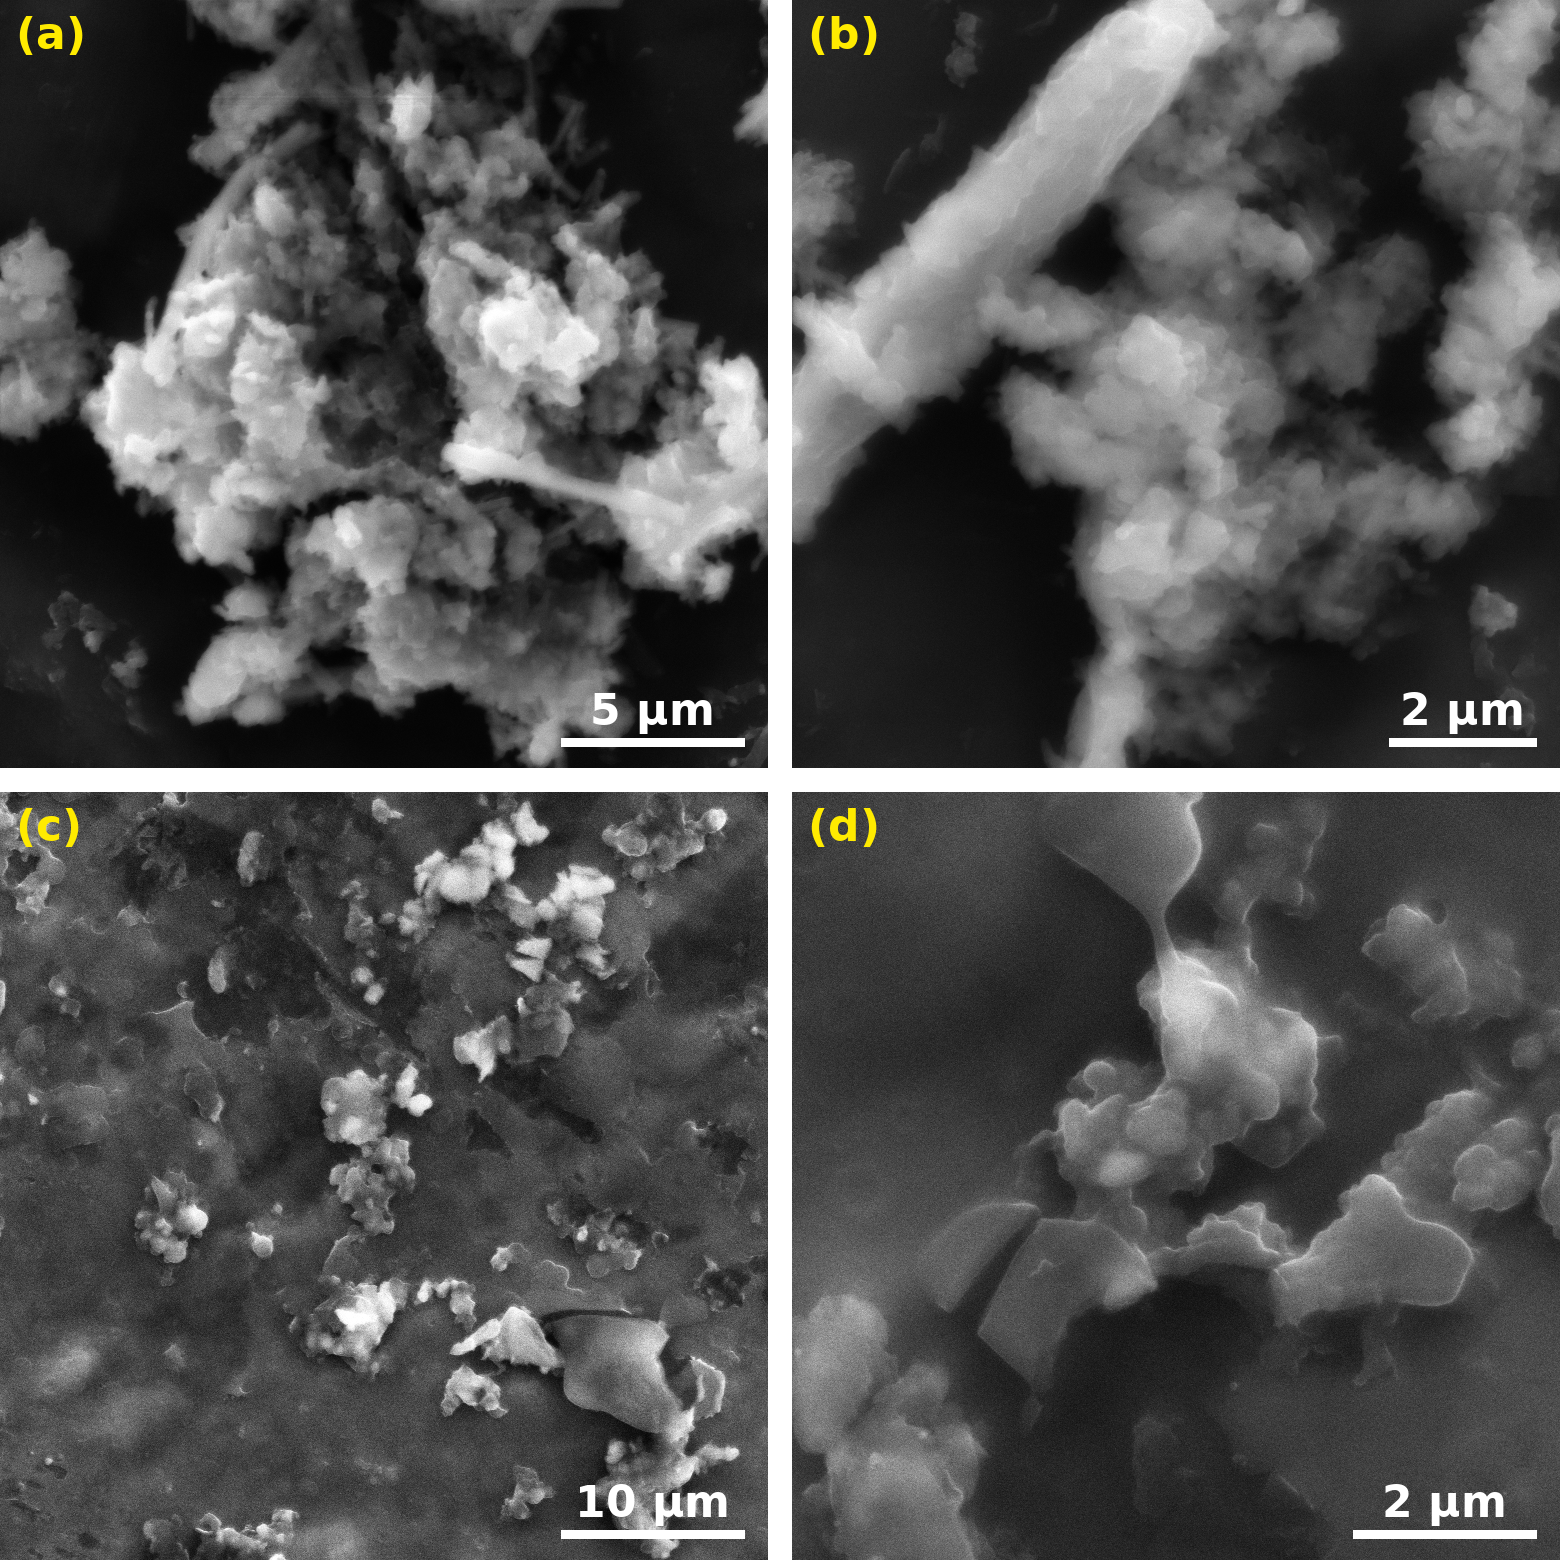
\includegraphics[width=0.72\linewidth]{Figure_4.png}
\caption{FESEM images of the precursor (a, b) and the composite (c, d).}
\label{fig:fesem}
\end{figure}

\Cref{fig:fesem} compares the hydrothermal precursor, imaged at 10\,000$\times$ and 20\,000$\times$ in panels (a) and (b), with the composite made from it, imaged at 5000$\times$ and 25\,000$\times$ in panels (c) and (d). The precursor (\Cref{fig:fesem}a, b) is a loose assembly of irregular agglomerates of fine particles, with a minority of straight rod- and ribbon-like crystallites among them. In the fields we imaged these rods are several micrometres long and roughly 0.5--2~$\mu$m wide. Rod-like growth is the habit usually associated with hydrothermally grown silver vanadate \cite{menezes2019agvo3,mai2010agvo3,yan2023agvo3breath}, although our rods are much thicker than the nanowires in those reports, and morphology on its own does not identify a phase.

The composite looks different (\Cref{fig:fesem}c, d). None of the 11 images we recorded of it shows a rod-like particle comparable to those of the precursor. We see instead rounded, smooth-surfaced lumps about 1--5~$\mu$m across, often fused into clusters and lying on a featureless film, together with occasional angular, plate-like fragments 1--3~$\mu$m across. The soft, blurred edges at higher magnification are consistent with beam charging of a poorly conducting organic material, so we did not attempt to measure primary particle sizes. A polymer coat would thicken and round the rods, but it would not remove their elongated shape, and we see no elongated objects beneath the film. The change in habit between the two powders indicates that the rod-forming inorganic phase was transformed during Step~3, in line with the XRD result of \Cref{sec:phase}.

\subsection{Chemical bonding (FTIR)}
\label{sec:ftir}
Diffraction and microscopy do not say which chemical groups are present, so we turned to infrared spectroscopy to see what the two powders contain.


\begin{figure}[!htb]
\centering
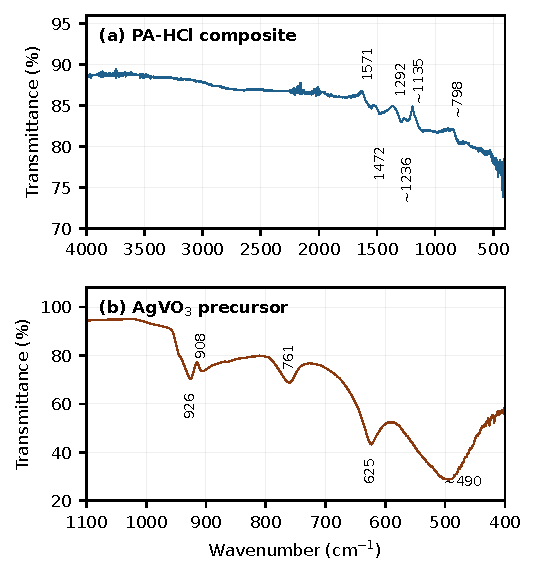
\includegraphics[width=0.62\linewidth]{Figure_5.pdf}
\caption{FTIR spectra of the composite (a) and the precursor (b).}
\label{fig:ftir}
\end{figure}

\Cref{fig:ftir} shows the two spectra and \Cref{tab:ftir} lists the band assignments. Panel (a) is the composite over the full range and panel (b) is the precursor from 1100~cm$^{-1}$ downwards, because the precursor has no notable bands above 1000~cm$^{-1}$; the numbers on the curves are band positions in cm$^{-1}$. We take the composite first. It shows the quinoid and benzenoid C=C stretching bands at 1571 and 1472~cm$^{-1}$, and having both at comparable depth is the defining signature of the emeraldine oxidation state \cite{yang2023panisensors,golba2019paniftir}. After a local baseline correction the quinoid-to-benzenoid band-height ratio is about 1.2, close to the value of one expected for emeraldine, with no sign that the polymer has been strongly over-oxidised. The bands at 1292 and about 1236~cm$^{-1}$ come from C--N and C--N$^{+\bullet}$ stretching, and the band at about 1141~cm$^{-1}$ is the B--NH$^{+}$=Q electronic-like band, whose presence is associated with the protonated, conducting state. The band at about 798~cm$^{-1}$ is the out-of-plane C--H bend of a 1,4-disubstituted ring, which points to head-to-tail para-coupling of the aniline units. The baseline of the spectrum falls steadily from about 89\% transmittance at 4000~cm$^{-1}$ to about 77\% near 450~cm$^{-1}$. This is the broad electronic absorption expected from delocalised charge carriers in conducting PANI, although scattering from the particles may also contribute. The bands are weak, only 1--2 percentage points deep, so we assign them on position and pattern and not on intensity. We see no distinct N--H or O--H stretching band between 3200 and 3500~cm$^{-1}$.

% Table 4: compiles on its own (pdflatex) and is also \input by main.tex.
\expandafter\ifx\csname documentclass\expandafter\endcsname\csname @notprerr\endcsname\else
\expandafter\ifx\csname documentclass\expandafter\endcsname\csname @twoclasseserror\endcsname\else
\documentclass[11pt]{article}
\usepackage[a4paper,landscape,margin=2cm]{geometry}
\usepackage[T1]{fontenc}
\usepackage[utf8]{inputenc}
\usepackage{times}
\usepackage{amsmath,amssymb}
\usepackage{booktabs,array,multirow,adjustbox,siunitx}
\newcolumntype{L}[1]{>{\raggedright\arraybackslash}p{#1}}
\expandafter\gdef\csname tabcite@ibrahim2024chitosanagvo3\endcsname{27}
\newcommand{\Cref}[1]{\csname tabref@#1\endcsname}
\renewcommand{\cite}[1]{[\csname tabcite@#1\endcsname]}
\pagestyle{empty}
\setlength{\parindent}{0pt}
\gdef\tabstandalone{1}
\begin{document}
\setcounter{table}{3}
\fi\fi
\begin{table}[!htbp]
\centering
\caption{FTIR band assignments.}
\label{tab:ftir}
\scriptsize
\begin{adjustbox}{max width=\textwidth,center}
\begin{tabular}{L{1.5cm}L{5.6cm}}
\toprule
\textbf{Band (cm$^{-1}$)} & \textbf{Assignment} \\
\midrule
\multicolumn{2}{l}{\emph{PA-HCl composite}} \\
1571 & C=C stretching, quinoid ring \\
1472 & C=C stretching, benzenoid ring \\
1292 & C--N stretching, secondary aromatic amine \\
$\sim$1236 & C--N$^{+\bullet}$ stretching (polaron) \\
$\sim$1141 & B--NH$^{+}$=Q electronic-like band (doped state) \\
$\sim$798 & C--H oop bending, 1,4-disubstituted ring \\
\midrule
\multicolumn{2}{l}{\emph{AgVO$_3$ precursor}} \\
926 & VO$_3$ symmetric stretching and V=O stretching \\
908 & Ag--O--V bridging or O--V--O vibration \\
761 & VO$_3$ antisymmetric stretching \\
625 & V--O--V stretching \\
$\sim$490 & Strong, broad lower-frequency vanadate band, cut off by the 400~cm$^{-1}$ limit; not assigned \\
\bottomrule
\end{tabular}
\end{adjustbox}
\\[3pt]
\begin{minipage}{0.96\linewidth}
\raggedright\scriptsize B = benzenoid ring, Q = quinoid ring, oop = out-of-plane bend. Bands marked $\sim$ are weak and uncertain to about $\pm$5~cm$^{-1}$, the others to about $\pm$2~cm$^{-1}$. Vanadate assignments follow the AgVO$_3$ bands of Ref.~\cite{ibrahim2024chitosanagvo3}.
\end{minipage}
\end{table}
\expandafter\ifx\csname tabstandalone\endcsname\relax\else
\end{document}
\fi


The precursor spectrum is quite different. Four sharp bands appear at 926, 908, 761 and 625~cm$^{-1}$, together with a strong, broad band centred near 490~cm$^{-1}$, and nothing else of note between 4000 and 1000~cm$^{-1}$, so no C--H or C=O absorption from organic residue. Ibrahim et~al.\ \cite{ibrahim2024chitosanagvo3} report AgVO$_3$ bands at 924, 891, 775 and 616~cm$^{-1}$ and assign them to the VO$_3$ symmetric stretch with V=O, Ag--O--V or O--V--O vibrations, the VO$_3$ antisymmetric stretch and V--O--V stretching. Our four bands match these to within 17~cm$^{-1}$ (926 against 924, 908 against 891, 761 against 775 and 625 against 616). We therefore assign them to a metavanadate of this type. The spectrum has no band near 1020~cm$^{-1}$, where the terminal V=O stretch of vanadium pentoxide is usually found, so a V$_2$O$_5$-type phase is unlikely. This supports a metavanadate-type precursor.

None of the four vanadate bands can be picked out in the composite spectrum. The composite spectrum is weak, and the 761 and 625~cm$^{-1}$ bands lie on the rising baseline close to the PANI band at 798~cm$^{-1}$. The absence of vanadate bands agrees with the XRD pattern of the composite, which contains no vanadate reflections (\Cref{sec:xrd}).

\subsection{Combined assessment of phase identity}
\label{sec:phase}

None of the characterisation techniques settles the question of phase identity on its own, so we consider them together.

\subsubsection{Diffraction}
All eight sharp reflections of the composite in \Cref{fig:xrd}b index to a single face-centred-cubic lattice, with (111), (200), (220), (311), (222), (400), (331) and (420) all present. We refined the lattice parameter and a zero offset together by weighted least squares over the eight fitted positions. This gives $a = 5.5544 \pm 0.0003$~\AA{} and an offset of $+0.142 \pm 0.002^{\circ}$, with every observed position reproduced to within 0.02$^{\circ}$ in 2$\theta$ (0.004$^{\circ}$ for seven of the eight). The value of $a$ is 0.10\% above the 5.549~\AA{} cell of chlorargyrite (AgCl). As a check, \Cref{eq:cubic} applied to each corrected reflection gives values between 5.5541 and 5.5557~\AA, consistent with the refined value. This is a complete assignment, with no unindexed sharp reflection left over. The relative intensities need one comment. The (220) line is slightly stronger than (111), whereas one expects (111) to be the stronger of the two in a randomly oriented powder, and we suggest preferred orientation of the cubic crystallites in the flat holder as a possible cause. We did not test this, and the assignment rests on the positions and not on the intensities. The pattern contains silver only in the form of AgCl.

The precursor pattern is a different matter. It has a dense set of reflections, several of them below 30$^{\circ}$, which is the signature of a low-symmetry phase with a large unit cell. The monoclinic cell of $\beta$-AgVO$_3$ ($a \approx 18.1$, $b \approx 3.58$, $c \approx 8.04$~\AA, $\beta \approx 104.4^{\circ}$) \cite{menezes2019agvo3} would give such a pattern, and the precursor does show a line at $d$ = 3.580~\AA, equal to the $b$ axis of that cell, together with a strong line at $d$ = 3.167~\AA{} close to the 0.317~nm lattice spacing that Gao et~al.\ assigned to $\beta$-AgVO$_3$ by electron microscopy \cite{gao2017ag3vo4agvo3}. We therefore describe the precursor as a crystalline silver vanadate of the low-symmetry type expected for $\beta$-AgVO$_3$; a full indexing against the reference card is left for the next stage. The precursor shows no sign of silver chloride in the form that matters here: the AgCl (311) position at 54.8$^{\circ}$ is empty, whereas it carries 16\% of the (200) intensity in the composite.

\subsubsection{Precursor identity}
FTIR, XRD and FESEM point to the same precursor: a crystalline silver metavanadate. It shows the vanadate bands at 926, 908, 761 and 625~cm$^{-1}$ (\Cref{sec:ftir}), a sharp, many-line, low-symmetry diffraction pattern (\Cref{fig:xrd}a) and rod-like crystallites (\Cref{sec:fesem}).

\subsubsection{Formation of AgCl in the acid step}
The composite pattern contains AgCl and no vanadate reflection, which follows from how we made it. In Step~3 the precursor sits in 40~mL of 1~M HCl at 0--5~$^{\circ}$C for several hours (\Cref{fig:synthesis}). That volume holds 40~mmol of chloride, whereas 100~mg of AgVO$_3$ (molar mass 206.8~g~mol$^{-1}$) contains at most 0.48~mmol of silver, so chloride is in roughly 80-fold excess. AgCl has a solubility product of the order of $10^{-10}$, so any Ag$^{+}$ released from the vanadate in the acid precipitates essentially quantitatively as AgCl. The vanadium(V) most likely dissolves at this acidity as VO$_2^{+}$ and leaves with the filtrate, which accounts for the absence of a vanadate band by FTIR and of rods by FESEM. We keep the name PANI--AgVO$_3$ for the material we set out to make and for its precursor. The crystalline inorganic component detected in the coating prepared in HCl is AgCl. PANI/AgCl composites formed in chloride-containing aqueous media have been reported before \cite{benahmed2018paniagcl,vohra2013agclpani}.

\subsection{Gas-sensing performance}
\label{sec:gassensing}
The characterisation tells us what we put on the sensor, namely the PANI--AgVO$_3$ coating prepared in hydrochloric acid (\Cref{sec:phase}). We now show how that coating changes the response of the MiCS-4514 to NO$_2$, VOC vapour, NH$_3$ and CO. The main element of each gas is the OX element for NO$_2$ and NH$_3$ and the RED element for VOC vapour and CO. In all eight runs the RED element started from a baseline resistance of 123--532~k$\Omega$, inside the window of 100--1500~k$\Omega$ that the manufacturer specifies \cite{sgx2019mics4514}, and at 13~ppm CO the coated RED element gave a resistance ratio of 0.43, in line with the typical value of about 0.42 read from the typical-sensitivity curve in the data sheet.

\subsection{Transient response}
\label{sec:transient}
\Cref{fig:transient} shows the resistance ratio $R_s/R_0$ of the main element of each gas through its whole run. The coated NO$_2$ trace stays near 1 up to 0.4~ppm and then climbs in clear steps to about 60 at 1~ppm, whereas the uncoated trace stays between 0.9 and 1.1 over the whole run (\Cref{fig:transient}a). The VOC traces of both sensors fall in steps to about 0.2 at 0.3~ppm, and the coated trace falls earlier and faster (\Cref{fig:transient}b). The NH$_3$ traces carry a regular ripple with a period of about 4~min, and the coated trace follows the concentration steps upwards (\Cref{fig:transient}c). The CO traces fall in steps to 0.43 (coated) and 0.34 (uncoated) at 13~ppm (\Cref{fig:transient}d). Each run covers the full concentration range in a single continuous exposure of 65 to 95~min.

\begin{figure}[!htbp]
\centering
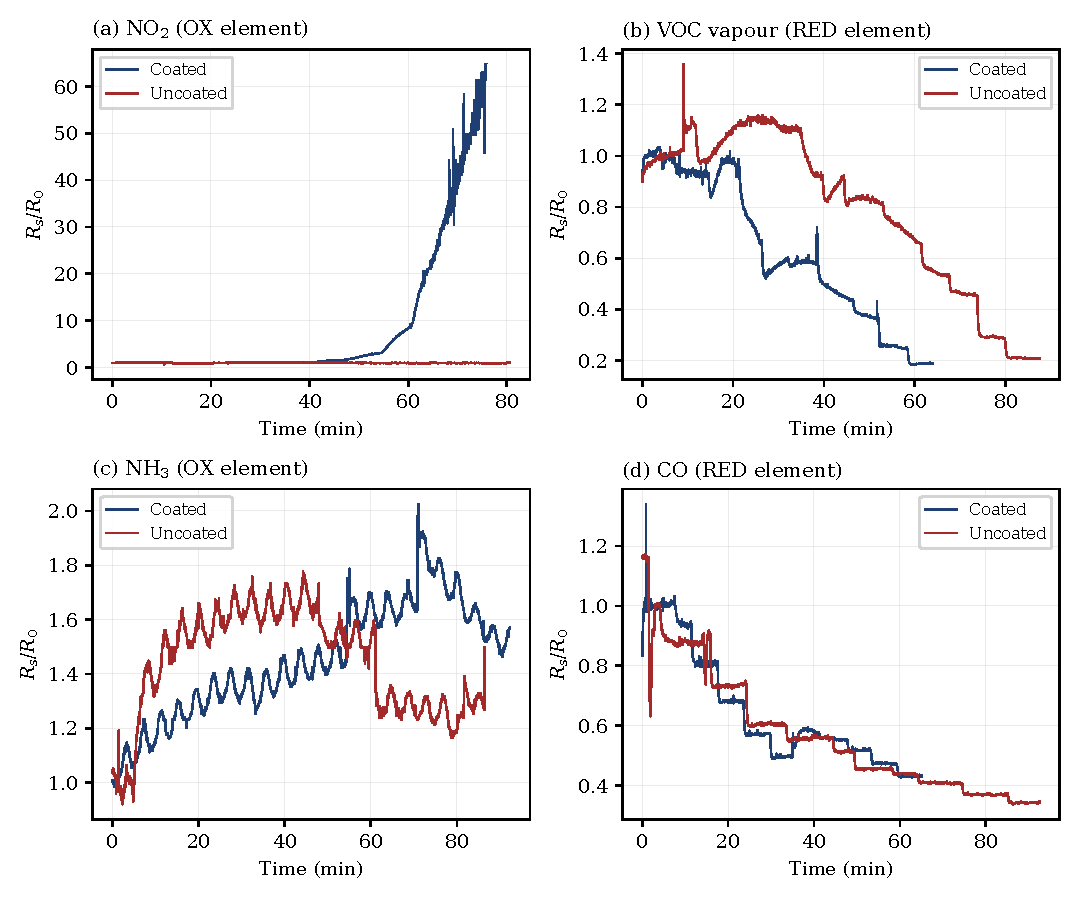
\includegraphics[width=0.95\textwidth]{Figure_6.pdf}
\caption{Resistance ratio $R_s/R_0$ over each run.}
\label{fig:transient}
\end{figure}

\subsection{Calibration curves}
\label{sec:calibration}
\Cref{fig:calibration} plots the step means of the sensitivity against the concentration for the main element of each gas, with the fits of \Cref{tab:fits}; the error bars are the standard deviation of the samples within each step. For NO$_2$ the coated sensor follows the power law $S=44.06\,C^{7.457}$ ($R^2=0.993$, \Cref{fig:calibration}a). The large exponent describes a threshold-like onset, with $S$ close to 1 up to 0.4~ppm and a steep rise above it, so we use the equation as an interpolation formula. The uncoated sensor stays at $S\approx 0.95$ over the whole range. For VOC vapour both sensors follow a sub-linear power law, $S=10.76\,C^{0.610}$ for the coated sensor ($R^2=0.982$) and $S=10.01\,C^{0.656}$ for the uncoated one ($R^2=0.972$), and the coated curve lies above the uncoated one over the whole range (\Cref{fig:calibration}b). The coated sensitivity for NH$_3$ rises steadily to 1.79 at 0.8~ppm, and a quadratic describes the curve with $R^2=0.934$, against $R^2=0.545$ for the uncoated sensor (\Cref{fig:calibration}c). For CO both sensors follow a sub-linear power law, with exponents of 0.242 (coated) and 0.471 (uncoated), and the coated curve lies above the uncoated one up to 7~ppm (\Cref{fig:calibration}d).

\begin{figure}[!htbp]
\centering
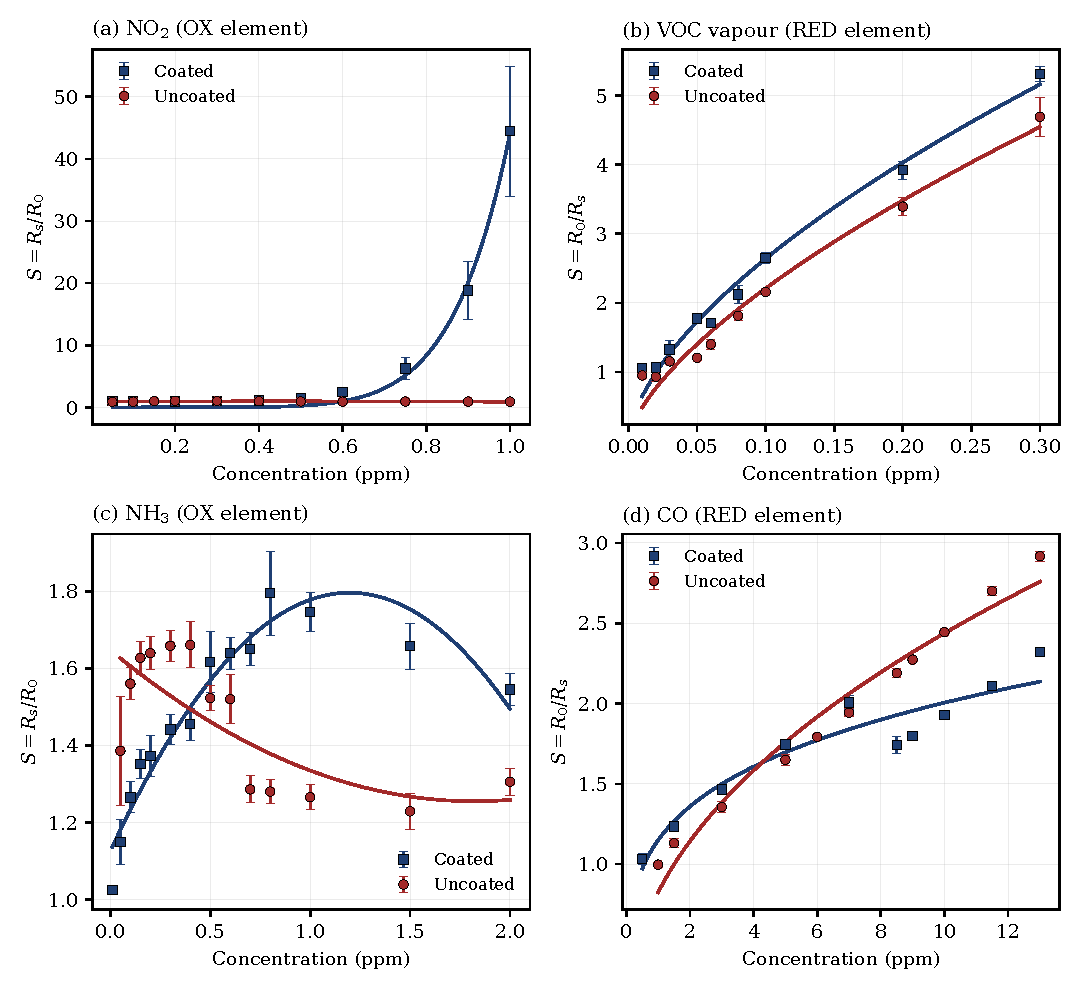
\includegraphics[width=0.95\textwidth]{Figure_7.pdf}
\caption{Sensitivity against concentration, with fits.}
\label{fig:calibration}
\end{figure}

% Table 5: compiles on its own (pdflatex) and is also \input by main.tex.
\expandafter\ifx\csname documentclass\expandafter\endcsname\csname @notprerr\endcsname\else
\expandafter\ifx\csname documentclass\expandafter\endcsname\csname @twoclasseserror\endcsname\else
\documentclass[11pt]{article}
\usepackage[a4paper,landscape,margin=2cm]{geometry}
\usepackage[T1]{fontenc}
\usepackage[utf8]{inputenc}
\usepackage{times}
\usepackage{amsmath,amssymb}
\usepackage{booktabs,array,multirow,adjustbox,siunitx}
\newcolumntype{L}[1]{>{\raggedright\arraybackslash}p{#1}}

\newcommand{\Cref}[1]{\csname tabref@#1\endcsname}
\renewcommand{\cite}[1]{[\csname tabcite@#1\endcsname]}
\pagestyle{empty}
\setlength{\parindent}{0pt}
\gdef\tabstandalone{1}
\begin{document}
\setcounter{table}{4}
\fi\fi
\begin{table}[!htbp]
\centering
\caption{Fits of the sensitivity $S$ to the concentration $C$ in ppm.}
\label{tab:fits}
\scriptsize
\setlength{\tabcolsep}{5pt}
\begin{adjustbox}{max width=\textwidth,center}
\begin{tabular}{llllcccc}
\toprule
\textbf{Gas} & \textbf{Element} & \textbf{Sensor} & \textbf{Model} & \textbf{Equation} & \textbf{$R^{2}$} & \textbf{RMSE} & \textbf{$n$} \\
\midrule
NO$_2$ & OX & Coated & Power law & $S=44.06\,C^{7.457}$ & 0.993 & 1.094 & 10 \\
NO$_2$ & OX & Uncoated & Quadratic & $S=-0.201C^2+0.163C+0.950$ & 0.216 & 0.040 & 11 \\
VOC vapour & RED & Coated & Power law & $S=10.76\,C^{0.610}$ & 0.982 & 0.182 & 9 \\
VOC vapour & RED & Uncoated & Power law & $S=10.01\,C^{0.656}$ & 0.972 & 0.204 & 9 \\
NH$_3$ & OX & Coated & Quadratic & $S=-0.468C^2+1.120C+1.126$ & 0.934 & 0.056 & 14 \\
NH$_3$ & OX & Uncoated & Quadratic & $S=0.118C^2-0.431C+1.647$ & 0.545 & 0.109 & 13 \\
CO & RED & Coated & Power law & $S=1.15\,C^{0.242}$ & 0.903 & 0.117 & 10 \\
CO & RED & Uncoated & Power law & $S=0.82\,C^{0.471}$ & 0.967 & 0.109 & 11 \\
\bottomrule
\end{tabular}
\end{adjustbox}
\\[3pt]
\begin{minipage}{0.7\textwidth}
\raggedright\scriptsize RMSE is the root-mean-square error and $n$ the number of concentration steps in the fit.
\end{minipage}
\end{table}
\expandafter\ifx\csname tabstandalone\endcsname\relax\else
\end{document}
\fi


\subsection{Resistance ratios}
\label{sec:ratio}
\Cref{fig:ratio} shows the same data in the form that the data sheet uses, the ratio $R_s/R_0$ against concentration on logarithmic axes. On the RED element (\Cref{fig:ratio}a) both CO and VOC vapour lower the resistance. The VOC curve of the coated sensor lies below that of the uncoated sensor at every concentration, which means a stronger response, and the CO curves coincide up to 7~ppm. On the OX element (\Cref{fig:ratio}b) the coated NO$_2$ ratio is near 1 up to 0.4~ppm and then climbs by more than an order of magnitude to 44 at 1~ppm, while the uncoated ratio stays between 0.9 and 1.1. Ammonia raises the resistance of the OX element in both sensors.

\begin{figure}[!htbp]
\centering
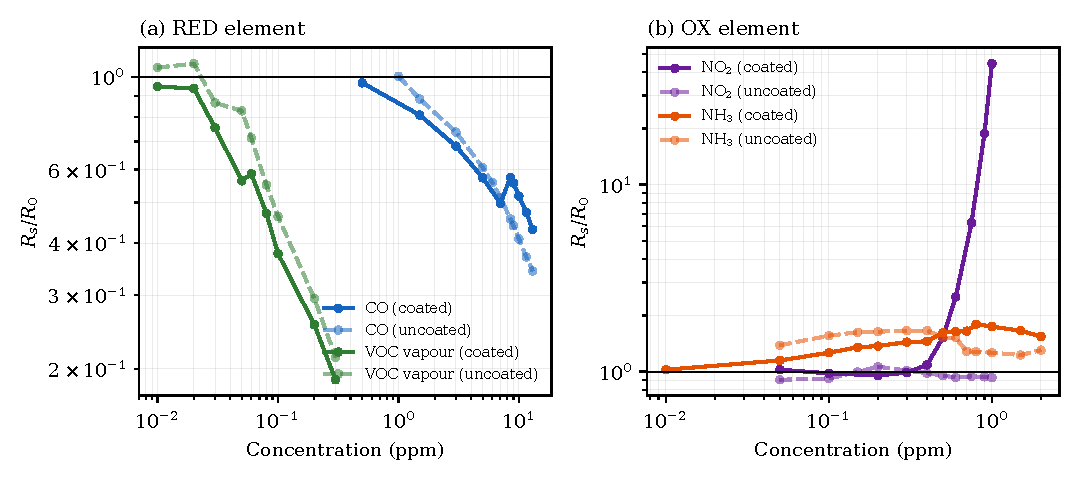
\includegraphics[width=0.9\textwidth]{Figure_8.pdf}
\caption{Resistance ratio $R_s/R_0$ against concentration.}
\label{fig:ratio}
\end{figure}

\subsection{Enhancement over the uncoated sensor}
\label{sec:ef}
\Cref{fig:enh} and \Cref{tab:enh} give the enhancement $E$ of \Cref{eq:enh} at every concentration at which both sensors were measured.

\begin{figure}[!htbp]
\centering
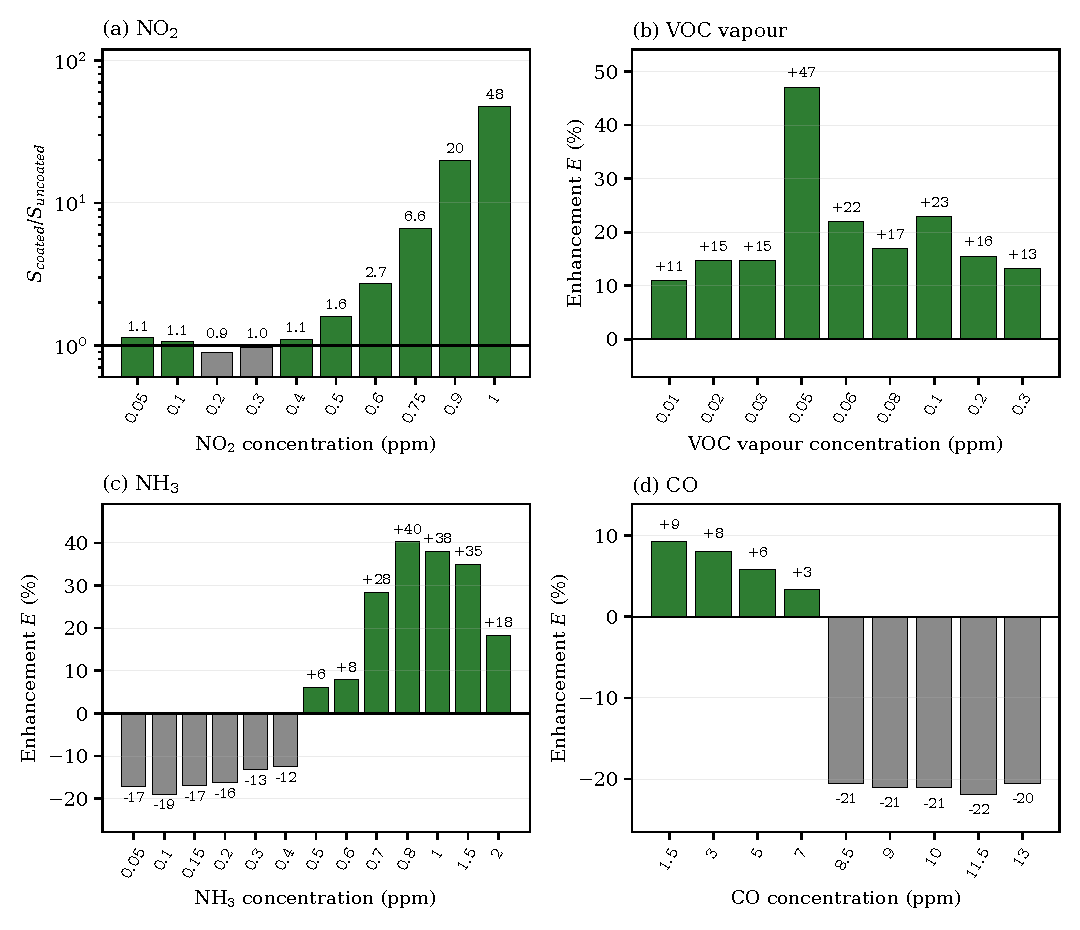
\includegraphics[width=0.95\textwidth]{Figure_9.pdf}
\caption{Enhancement of the coated over the uncoated sensor.}
\label{fig:enh}
\end{figure}

The VOC response of the coated sensor is higher than that of the uncoated sensor at all nine concentrations, by 11 to 47\% with a median of 16\%, and the largest gain, 47\%, is at 0.05~ppm (\Cref{fig:enh}b). For NO$_2$ the enhancement factor, shown on a logarithmic axis, grows steadily from 0.4~ppm: 1.1, 1.6, 2.7, 6.6, 20 and 47.8 at 0.4, 0.5, 0.6, 0.75, 0.9 and 1~ppm (\Cref{fig:enh}a). The uncoated OX element stayed at $S\approx 0.93$--1.06 over this range and the two OX elements started from different baseline resistances, so replicate devices will be used to confirm the size of this factor. For NH$_3$ the coated sensor responds more strongly from 0.5~ppm, by 6 and 8\% at 0.5 and 0.6~ppm and by 28 to 40\% from 0.7 to 1.5~ppm (the uncoated OX baseline in this run was 88~$\Omega$, against 3.8--4.4~k$\Omega$ in the NO$_2$ and VOC runs), with a maximum of $+40$\% at 0.8~ppm and $+18$\% at 2~ppm; below 0.5~ppm the two sensors differ by $-12$ to $-19$\% (\Cref{fig:enh}c). For CO the coated sensor is higher by 9, 8, 6 and 3\% at 1.5, 3, 5 and 7~ppm, and the uncoated sensor is higher by 20--22\% from 8.5 to 13~ppm (\Cref{fig:enh}d).

% Table 6: compiles on its own (pdflatex) and is also \input by main.tex.
\expandafter\ifx\csname documentclass\expandafter\endcsname\csname @notprerr\endcsname\else
\expandafter\ifx\csname documentclass\expandafter\endcsname\csname @twoclasseserror\endcsname\else
\documentclass[11pt]{article}
\usepackage[a4paper,landscape,margin=2cm]{geometry}
\usepackage[T1]{fontenc}
\usepackage[utf8]{inputenc}
\usepackage{times}
\usepackage{amsmath,amssymb}
\usepackage{booktabs,array,multirow,adjustbox,siunitx}
\newcolumntype{L}[1]{>{\raggedright\arraybackslash}p{#1}}
\expandafter\gdef\csname tabref@eq:S\endcsname{Equation (2)}
\expandafter\gdef\csname tabref@eq:enh\endcsname{Equation (4)}
\newcommand{\Cref}[1]{\csname tabref@#1\endcsname}
\renewcommand{\cite}[1]{[\csname tabcite@#1\endcsname]}
\pagestyle{empty}
\setlength{\parindent}{0pt}
\gdef\tabstandalone{1}
\begin{document}
\setcounter{table}{5}
\fi\fi
\begin{table}[!htbp]
\centering
\caption{Sensitivity $S$ of the coated and uncoated sensors and the enhancement $E$ at each tested concentration.}
\label{tab:enh}
\scriptsize
\setlength{\tabcolsep}{3.2pt}
\begin{adjustbox}{max width=\textwidth,center}
\begin{tabular}{rrrr@{\hspace{14pt}}rrrr@{\hspace{14pt}}rrrr@{\hspace{14pt}}rrrr}
\toprule
\multicolumn{4}{c}{\textbf{NO$_2$ (OX)}} & \multicolumn{4}{c}{\textbf{VOC vapour (RED)}} & \multicolumn{4}{c}{\textbf{NH$_3$ (OX)}} & \multicolumn{4}{c}{\textbf{CO (RED)}} \\
\cmidrule(r{8pt}){1-4}\cmidrule(r{8pt}){5-8}\cmidrule(r{8pt}){9-12}\cmidrule{13-16}
$C$ & Coated & Uncoated & $E$ & $C$ & Coated & Uncoated & $E$ & $C$ & Coated & Uncoated & $E$ & $C$ & Coated & Uncoated & $E$ \\
(ppm) & $S$ & $S$ & (\%) & (ppm) & $S$ & $S$ & (\%) & (ppm) & $S$ & $S$ & (\%) & (ppm) & $S$ & $S$ & (\%) \\
\midrule
0.05 & 1.03 & 0.91 & +13 & 0.01 & 1.05 & 0.95 & +11 & 0.01 & 1.03 & -- & -- & 0.5 & 1.03 & -- & -- \\
0.1 & 0.98 & 0.92 & +6 & 0.02 & 1.07 & 0.93 & +15 & 0.05 & 1.15 & 1.39 & -17 & 1 & -- & 1.00 & -- \\
0.15 & -- & 1.00 & -- & 0.03 & 1.32 & 1.15 & +15 & 0.1 & 1.27 & 1.56 & -19 & 1.5 & 1.23 & 1.13 & +9 \\
0.2 & 0.96 & 1.06 & -10 & 0.05 & 1.77 & 1.21 & +47 & 0.15 & 1.35 & 1.63 & -17 & 3 & 1.46 & 1.36 & +8 \\
0.3 & 0.99 & 1.02 & -3 & 0.06 & 1.71 & 1.40 & +22 & 0.2 & 1.37 & 1.64 & -16 & 5 & 1.75 & 1.65 & +6 \\
0.4 & 1.09 & 0.98 & +11 & 0.08 & 2.12 & 1.81 & +17 & 0.3 & 1.44 & 1.66 & -13 & 6 & -- & 1.79 & -- \\
0.5 & 1.52 & 0.95 & +60 & 0.1 & 2.65 & 2.16 & +23 & 0.4 & 1.45 & 1.66 & -12 & 7 & 2.01 & 1.94 & +3 \\
0.6 & 2.52 & 0.93 & +170 & 0.2 & 3.92 & 3.39 & +16 & 0.5 & 1.62 & 1.52 & +6 & 8.5 & 1.74 & 2.19 & -21 \\
0.75 & 6.26 & 0.95 & +562 & 0.3 & 5.31 & 4.69 & +13 & 0.6 & 1.64 & 1.52 & +8 & 9 & 1.80 & 2.27 & -21 \\
0.9 & 18.81 & 0.94 & +1902 &  &  &  &  & 0.7 & 1.65 & 1.29 & +28 & 10 & 1.93 & 2.44 & -21 \\
1 & 44.46 & 0.93 & +4679 &  &  &  &  & 0.8 & 1.79 & 1.28 & +40 & 11.5 & 2.11 & 2.70 & -22 \\
 &  &  &  &  &  &  &  & 1 & 1.75 & 1.27 & +38 & 13 & 2.32 & 2.92 & -20 \\
 &  &  &  &  &  &  &  & 1.5 & 1.66 & 1.23 & +35 &  &  &  &  \\
 &  &  &  &  &  &  &  & 2 & 1.55 & 1.31 & +18 &  &  &  &  \\
\bottomrule
\end{tabular}
\end{adjustbox}
\\[3pt]
\begin{minipage}{0.96\textwidth}
\raggedright\scriptsize $S$ is the step-mean sensitivity of \Cref{eq:S}; $E$ is the enhancement of \Cref{eq:enh}. A dash means that the concentration was not applied to one of the two sensors.
\end{minipage}
\end{table}
\expandafter\ifx\csname tabstandalone\endcsname\relax\else
\end{document}
\fi



\subsection{Selectivity}
\label{sec:selectivity}
\Cref{fig:select} compares the largest sensitivity reached for each gas, on a logarithmic axis. The coated sensor gave 44.5 for NO$_2$ at 1~ppm, 5.31 for VOC vapour at 0.3~ppm, 2.32 for CO at 13~ppm and 1.79 for NH$_3$ at 0.8~ppm, so that the ratio to the NO$_2$ value is 0.119 for VOC vapour, 0.052 for CO and 0.040 for NH$_3$ (\Cref{tab:summary}). The NO$_2$ response is thus at least eight times each of the others. The concentration ranges differ (0.3~ppm for VOC vapour against 13~ppm for CO) and $S_{\mathrm{OX}}$ and $S_{\mathrm{RED}}$ come from different elements, so \Cref{fig:select} shows which response is largest in our test windows and not which gas the sensor prefers at equal concentration. The uncoated sensor gave 1.06, 4.67, 2.92 and 1.66 for the same four gases.

\begin{figure}[!htbp]
\centering
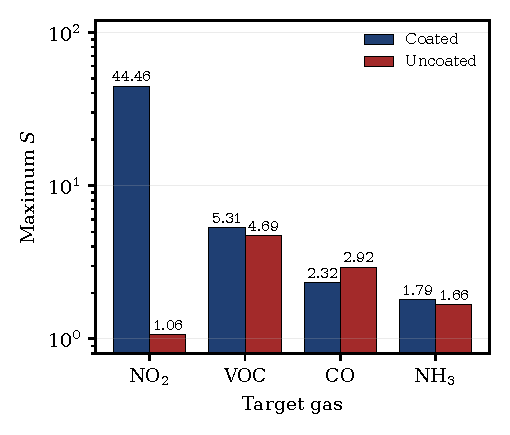
\includegraphics[width=0.8\linewidth]{Figure_10.pdf}
\caption{Largest sensitivity reached for each gas.}
\label{fig:select}
\end{figure}

\subsection{Reading the results together}
\label{sec:discussion}
Three results stand out. The coated OX element gives the largest and most concentration-sensitive response of the study, a threshold-like NO$_2$ response that starts at 0.4~ppm and reaches a sensitivity of 44.5 at 1~ppm. The VOC response is the most consistent gain: it is positive at all nine concentrations, both RED elements sit inside the specified baseline window, and the traces show clean steps. The NH$_3$ response of the OX element is higher than that of the uncoated sensor from 0.5~ppm, where the coated curve rises to its maximum of 1.79 at 0.8~ppm. At low concentration the coated CO response also follows or exceeds that of the uncoated sensor. Taken together, the coating adds NO$_2$, VOC and NH$_3$ functions to the commercial part.

\subsection{Summary of the sensing results}
\label{sec:summary}
\Cref{tab:summary} condenses the four gas results before we place them in the context of the literature.

% Table 7: compiles on its own (pdflatex) and is also \input by main.tex.
\expandafter\ifx\csname documentclass\expandafter\endcsname\csname @notprerr\endcsname\else
\expandafter\ifx\csname documentclass\expandafter\endcsname\csname @twoclasseserror\endcsname\else
\documentclass[11pt]{article}
\usepackage[a4paper,landscape,margin=2cm]{geometry}
\usepackage[T1]{fontenc}
\usepackage[utf8]{inputenc}
\usepackage{times}
\usepackage{amsmath,amssymb}
\usepackage{booktabs,array,multirow,adjustbox,siunitx}
\newcolumntype{L}[1]{>{\raggedright\arraybackslash}p{#1}}
\expandafter\gdef\csname tabref@eq:S\endcsname{Equation (2)}
\expandafter\gdef\csname tabref@tab:fits\endcsname{Table 5}
\newcommand{\Cref}[1]{\csname tabref@#1\endcsname}
\renewcommand{\cite}[1]{[\csname tabcite@#1\endcsname]}
\pagestyle{empty}
\setlength{\parindent}{0pt}
\gdef\tabstandalone{1}
\begin{document}
\setcounter{table}{6}
\fi\fi
\begin{table}[!htbp]
\centering
\caption{Summary of the sensing results for the main element of each gas.}
\label{tab:summary}
\scriptsize
\setlength{\tabcolsep}{4pt}
\begin{adjustbox}{max width=\textwidth,center}
\begin{tabular}{llccccL{5.4cm}}
\toprule
\textbf{Gas} & \textbf{Element} & \shortstack{\textbf{Coated}\\\textbf{$S_{\max}$}} & \shortstack{\textbf{Uncoated}\\\textbf{$S_{\max}$}} & \shortstack{\textbf{Ratio to}\\\textbf{NO$_2$}} & \shortstack{\textbf{Coated fit}\\\textbf{$R^{2}$}} & \textbf{Observation} \\
\midrule
NO$_2$ & OX & 44.46 & 1.06 & 1.000 & 0.993 & Threshold-like onset above 0.4~ppm; 47.8$\times$ at 1~ppm \\
VOC vapour & RED & 5.31 & 4.67 & 0.119 & 0.982 & Higher at all 9 steps ($+11$ to $+47$\%) \\
NH$_3$ & OX & 1.79 & 1.66 & 0.040 & 0.934 & Higher from 0.5~ppm ($+6$ to $+40$\%) \\
CO & RED & 2.32 & 2.92 & 0.052 & 0.903 & Higher up to 7~ppm ($+3$ to $+9$\%) \\
\bottomrule
\end{tabular}
\end{adjustbox}
\\[3pt]
\begin{minipage}{0.92\textwidth}
\raggedright\scriptsize $S_{\max}$ is the largest step sensitivity of \Cref{eq:S} over the tested range (1~ppm NO$_2$, 0.3~ppm VOC vapour, 0.8~ppm for the NH$_3$ maximum of the coated sensor, 13~ppm CO); the uncoated maximum for NH$_3$ is at 0.4~ppm. The ratio to NO$_2$ is that of the coated $S_{\max}$ values. The fit $R^2$ is that of the coated sensor in \Cref{tab:fits}.
\end{minipage}
\end{table}
\expandafter\ifx\csname tabstandalone\endcsname\relax\else
\end{document}
\fi


\subsection{Comparison with the literature}
\label{sec:comparison}
To place the results in context, we finally set them beside published gas sensors.

\Cref{tab:comparison} puts our results next to the published work, with two cautions. First, response is defined differently across these studies (a percentage sensitivity per ppm, a percentage change, a plain resistance ratio, or the relative resistance change $S$ we use), so the response column cannot be compared directly between rows. Second, the platforms differ. Every literature entry uses a purpose-built transducer, whereas we coat a packaged commercial MOX part, which fixes the electrode geometry, operating temperature and baseline resistance.

% Table 8: compiles on its own (pdflatex) and is also \input by main.tex.
\expandafter\ifx\csname documentclass\expandafter\endcsname\csname @notprerr\endcsname\else
\expandafter\ifx\csname documentclass\expandafter\endcsname\csname @twoclasseserror\endcsname\else
\documentclass[11pt]{article}
\usepackage[a4paper,landscape,margin=2cm]{geometry}
\usepackage[T1]{fontenc}
\usepackage[utf8]{inputenc}
\usepackage{times}
\usepackage{amsmath,amssymb}
\usepackage{booktabs,array,multirow,adjustbox,siunitx}
\newcolumntype{L}[1]{>{\raggedright\arraybackslash}p{#1}}
\expandafter\gdef\csname tabref@eq:S\endcsname{Equation (2)}
\expandafter\gdef\csname tabcite@bonyani2022auzno\endcsname{12}
\expandafter\gdef\csname tabcite@chu2023ga2o3\endcsname{4}
\expandafter\gdef\csname tabcite@guo2021sno2zno\endcsname{3}
\expandafter\gdef\csname tabcite@mai2010agvo3\endcsname{21}
\expandafter\gdef\csname tabcite@saeed2024chitosansal\endcsname{19}
\expandafter\gdef\csname tabcite@singh2023hcn\endcsname{18}
\expandafter\gdef\csname tabcite@sonker2016panizno\endcsname{11}
\expandafter\gdef\csname tabcite@verma2024agcupani\endcsname{15}
\expandafter\gdef\csname tabcite@yan2023agvo3breath\endcsname{22}
\expandafter\gdef\csname tabcite@zhang2020panisrge\endcsname{10}
\expandafter\gdef\csname tabcite@zhou2024ternary\endcsname{16}
\newcommand{\Cref}[1]{\csname tabref@#1\endcsname}
\renewcommand{\cite}[1]{[\csname tabcite@#1\endcsname]}
\pagestyle{empty}
\setlength{\parindent}{0pt}
\gdef\tabstandalone{1}
\begin{document}
\setcounter{table}{7}
\fi\fi
\begin{table}[!htbp]
\centering
\caption{Comparison with published gas sensors.}
\label{tab:comparison}
\scriptsize
\setlength{\tabcolsep}{3pt}
\begin{adjustbox}{max width=\textwidth,center}
\begin{tabular}{L{3.3cm}L{1.4cm}L{1.3cm}L{1.1cm}L{2.3cm}L{2.6cm}L{1.4cm}L{1.4cm}L{1.1cm}}
\toprule
\textbf{Sensing material} & \textbf{Target gas} & \textbf{Conc.} & \textbf{Temp.} & \textbf{Platform} & \textbf{Response} & \textbf{Response time} & \textbf{Recovery time} & \textbf{Ref.} \\
\midrule
\multicolumn{9}{l}{\textit{This work (coated MiCS-4514, highest tested concentration unless noted)}} \\
PANI--AgVO$_3$ on MiCS-4514 & NO$_2$ & 1.0 ppm & RT & Commercial metal-oxide sensor, coated & $S_{OX}$ = 44.5 (uncoated 0.93$^{b}$) & NR & NR & This work \\
PANI--AgVO$_3$ on MiCS-4514 & VOC vapour & 0.3 ppm & RT & Commercial metal-oxide sensor, coated & $S_{RED}$ = 5.31 (uncoated 4.67) & NR & NR & This work \\
PANI--AgVO$_3$ on MiCS-4514 & NH$_3$ & 0.8 ppm$^{a}$ & RT & Commercial metal-oxide sensor, coated & $S_{OX}$ = 1.79 (uncoated 1.28) & NR & NR & This work \\
PANI--AgVO$_3$ on MiCS-4514 & CO & 13 ppm & RT & Commercial metal-oxide sensor, coated & $S_{RED}$ = 2.32 (uncoated 2.92) & NR & NR & This work \\
\midrule
\multicolumn{9}{l}{\textit{Published work (as reported by the original authors)}} \\
$\beta$-AgVO$_3$ nanowire (single) & H$_2$S & 50 ppm & RT & Single-nanowire device & Selective; 6 V threshold switching & $<$20 s & $<$20 s & \cite{mai2010agvo3} \\
AgVO$_3$ nanowires & Humidity & 20--90\% RH & RT & Gold interdigitated electrode on polyimide & $\sim$1 order of magnitude change in resistance & 0.6 s & 1.2 s & \cite{yan2023agvo3breath} \\
PANI/SrGe$_4$O$_9$ & NH$_3$ & 0.2 ppm & 25 $^{\circ}$C & Flexible interdigitated electrode & 16\% (8\% for PANI); detection limit 250 ppt & 24 s$^{b}$ & NR & \cite{zhang2020panisrge} \\
PANI@Ag/Cu & NH$_3$ & 300 ppm & RT & Resistive film & 86\% & NR & NR & \cite{verma2024agcupani} \\
PANI/copper phthalocyanine/silver nanoparticles & NH$_3$ & 500 ppm & RT & Flexible film, wireless read-out & 3.6; detection limit 0.234 ppm & 61 s & 19 s & \cite{zhou2024ternary} \\
PANI/montmorillonite--reduced graphene oxide & HCN & 2 ppm & RT & Resistive film & 4.56\%; 1.1174 ppm$^{-1}$ & NR & NR & \cite{singh2023hcn} \\
PANI--ZnO (5 wt\% PANI) & NO$_2$ & 20 ppm & RT & Thin film & $\sim$611 & NR & NR & \cite{sonker2016panizno} \\
Au/ZnO nanofibres coated with PANI & NO$_2$ & 50 ppm & 300 $^{\circ}$C & Electrospun nanofibres & $\sim$50 & NR & NR & \cite{bonyani2022auzno} \\
Hollow SnO$_2$/ZnO nanofibres & NO$_2$ & 0.5 ppm & $\sim$20 $^{\circ}$C & Screen-printed Ag, flexible & 336\% (13\% for SnO$_2$) & NR & NR & \cite{guo2021sno2zno} \\
Ga$_2$O$_3$ nanorods & NO$_2$ & 10 ppm & NR & Seeded substrate & 1184.6\%; 34.2\% at 100 ppb & 63.6 s & 135.7 s & \cite{chu2023ga2o3} \\
Chitosan--salicylaldehyde/$\beta$-cyclodextrin/ZnO & NH$_3$ & 10 ppm & RT & Polymer composite film & 6192 (712 unmodified); detection limit 0.12 ppb & 650 s & 350 s & \cite{saeed2024chitosansal} \\
\bottomrule
\end{tabular}
\end{adjustbox}
\\[3pt]
\begin{minipage}{0.96\textwidth}
\raggedright\scriptsize \textbf{Notes.} $S_{RED}$ and $S_{OX}$ are the sensitivity factors of the reducing and oxidising elements of the MiCS-4514 (\Cref{eq:S}); the value for the uncoated sensor at the same concentration is given in brackets. Values for published work are quoted as reported (percentage change, ratio, voltage or current), so a number in one row cannot be set directly against another. Conc.\ is the tested gas concentration (ppm, ppb and ppt are parts per million, billion and trillion), Temp.\ the operating temperature, RT room temperature, RH relative humidity, NR not reported, PANI polyaniline and VOC volatile organic compound. Response and recovery times are those reported at the stated concentration. $^{a}$ Concentration of the largest NH$_3$ response of the coated OX element. $^{b}$ No measurable change of the uncoated OX element over 0.05--1 ppm NO$_2$. Response and recovery times will be taken in cyclic exposures.
\end{minipage}
\end{table}
\expandafter\ifx\csname tabstandalone\endcsname\relax\else
\end{document}
\fi


Three points stand out. The materials with the highest reported responses get there through deliberate nanostructuring that maximises accessible surface area, namely hollow fibres \cite{guo2021sno2zno}, nanorod arrays \cite{chu2023ga2o3} and hierarchical mesoporous composites \cite{zhang2020panisrge}, whereas our coating is a drop-cast powder applied to a finished commercial part, and it still produces a large NO$_2$ response. The studies that show a gain from a composite all report the response of the unmodified component under identical conditions (8\% versus 16\% \cite{zhang2020panisrge} and 13\% versus 336\% \cite{guo2021sno2zno}), and our uncoated MiCS-4514 control provides the same kind of reference. Against that reference the coating gives a gain for VOC vapour at all tested concentrations (11 to 47\%), for NH$_3$ from 0.5~ppm (6 to 40\%), for NO$_2$ above 0.4~ppm and for CO up to 7~ppm (3 to 9\%). Finally, the stepped exposure used here has no recovery segments, and cyclic exposures will supply the response and recovery times that the table leaves open.

\subsection{Proposed sensing mechanism}
\label{sec:mechanism}
The measurements show what the coated sensor does, and this subsection gives our reading of why.

\begin{figure}[!htbp]
\centering
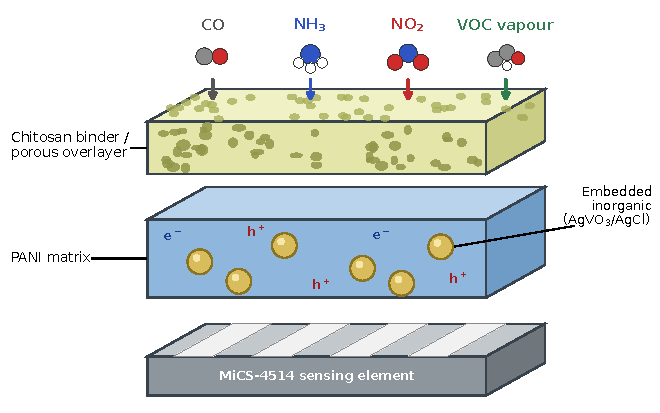
\includegraphics[width=0.85\linewidth]{Figure_11.pdf}
\caption{Proposed sensing mechanism. Schematic redrawn as vector graphics from a Google Gemini draft.}
\label{fig:mechanism}
\end{figure}

\Cref{fig:mechanism} sketches the coated sensing stack from the top. The test gases (CO, NH$_3$, NO$_2$ and VOC vapour) arrive from above and first meet the porous chitosan binder layer. Below it, the PANI matrix holds the embedded inorganic particles and exchanges electrons (e$^{-}$) and holes (h$^{+}$) with the adsorbed gases, and at the bottom sits the MiCS-4514 sensing element that carries the signal. PANI is a protonated, intrinsically conducting polymer whose conductivity responds to redox and acid--base interactions at its surface. A reducing or oxidising species donates electron density to the backbone or withdraws it and changes the resistivity, and for ammonia the response goes through deprotonation of the $-$NH$^{+}$= sites of the emeraldine salt \cite{yang2023panisensors}. The MiCS-4514 elements beneath the coating respond through the usual oxygen-vacancy and chemisorbed-oxygen mechanism of an $n$-type metal oxide \cite{fine2010mox}. Our results are compatible with both mechanisms operating together. CO and VOC vapour lower the resistance of the RED element, which points to the oxide element as the transducer, and the coating raises the VOC response throughout the tested range. Ammonia raises the resistance of the OX element, and the deprotonation route of the PANI layer adds to this response, which fits the higher sensitivity of the coated sensor from 0.5~ppm. For NO$_2$ the coated OX element shows a threshold-like onset above 0.4~ppm, and an interface between the polymer and the oxide that deepens the depletion layer is a plausible origin of the steep rise, as proposed for other PANI--oxide NO$_2$ sensors \cite{bonyani2022auzno}. The embedded inorganic particles in the schematic are labelled AgVO$_3$ for the intended phase, with the AgCl found in the composite discussed in \Cref{sec:phase}.

We keep the interpretation to what the data support. We made no band-alignment, work-function or oxidation-state measurement on this batch, so we do not assign the response to a particular p--n heterojunction, and a chitosan-only control will be measured next. \Cref{fig:mechanism} is therefore a literature-informed hypothesis that the measurements of the next stage can test.

% ====================================================================
\FloatBarrier
\section{Industrial Significance}
\label{sec:industrial}
% ====================================================================
We first comment on why the fabrication route matters.

The chitosan-stabilised drop-cast route we demonstrate is simple, uses very little material (1~$\mu$L per device) and is compatible with an existing commercial MOX package. The coated device survived the thermal budget of the sensor and a 24--28~h powered burn-in without loss of function. That practical result stands on its own: a coating step that costs a microlitre of ink and no change to the transducer is a realistic manufacturing addition.

At the present stage this is a \emph{demonstrated fabrication capability}. Environmental monitoring, occupational CO and NO$_2$ safety, and low-power IoT air-quality nodes remain the motivation for the further validation described in \Cref{sec:limitations}.

% ====================================================================
\FloatBarrier
\section{Limitations}
\label{sec:limitations}
The results above come from a first complete dataset, and the next steps are grouped by what they concern.

% ====================================================================
\subsection{Material and characterisation}
The precursor is identified as a crystalline silver metavanadate-type phase from its FTIR bands, its rod-like crystallites and its XRD pattern; indexing the full pattern against the reference card, and an elemental analysis of the precursor and the composite (for example by inductively coupled plasma optical emission spectroscopy), are the next steps for fixing the phase and the Ag:V and Ag:Cl ratios. The composite contains AgCl as its crystalline inorganic component (\Cref{sec:phase}), and testing other acid media will show whether the vanadate can be retained. The PANI loading and the polymer--particle interface were not measured, and a chitosan-only control coating is still to be recorded, since chitosan itself interacts with ammonia \cite{saeed2024chitosansal}.

\subsection{Device and measurement}
We tested one coated device and one uncoated control, with each concentration measured once, so replicate devices with matched baseline resistances will confirm the enhancement factors and define the device-to-device spread. The uncoated OX baseline also differed between runs (88~$\Omega$ in the NH$_3$ run against 3.8--4.4~k$\Omega$ in the NO$_2$ and VOC runs), so the NH$_3$ enhancement values are indicative and will be confirmed on fresh control devices. With the 3.3~V bias and the 220~$\Omega$ load, the power in the OX element was about 11--12~mW at the coated baseline, above the 8~mW rating of the data sheet \cite{sgx2019mics4514}, and it fell as the resistance rose during NO$_2$ exposure; the coated device worked through the burn-in and the test series. Each step lasted about 6~min with no gas-off segments, so response and recovery times will come from cyclic exposures, and limits of detection will follow from repeated blank measurements. The NH$_3$ traces carry a regular ripple with a period of about 4~min on both devices, which the repeat runs will also examine.

\subsection{Test conditions}
All measurements were made at a single nominal humidity (50\% RH) and at chamber temperatures of 22--28~$^{\circ}$C, so the humidity dependence remains to be measured, which matters because metal-oxide sensors drift with ambient temperature and humidity \cite{abdullah2022drift} and AgVO$_3$ nanowires are themselves effective humidity sensors \cite{yan2023agvo3breath}.

% ====================================================================
\section{Conclusion}
\label{sec:conclusion}
% ====================================================================
We coated a commercial MiCS-4514 gas sensor, which has two metal-oxide semiconductor sensing elements, with a polyaniline composite built on a silver vanadate precursor and applied as a chitosan-stabilised ink. The coating survived deposition, drying and a 24--28~h burn-in, and an identical uncoated sensor served as the control.

The precursor showed infrared bands at 926, 908, 761 and 625~cm$^{-1}$, rod-like crystallites and a many-line diffraction pattern. The composite prepared in 1~M hydrochloric acid contained polyaniline in its emeraldine-salt form and, by X-ray diffraction, silver chloride with a lattice parameter of $5.5544 \pm 0.0003$~\AA, which we attribute to the silver of the vanadate precipitating as AgCl in the acid step.

Against nitrogen dioxide, ammonia, carbon monoxide and volatile organic compounds at a nominal 50\% relative humidity, we expressed the response with the data-sheet sensitivity factors, each referred to the clean-air baseline of its own run. The coated sensor gave a sensitivity of 44.5 for 1~ppm nitrogen dioxide, described by the power law $S = 44.06\,C^{7.457}$ ($R^{2}=0.993$) with a threshold-like onset above 0.4~ppm, against 0.93 for the uncoated sensor, which gives an enhancement factor of 47.8. For volatile organic compound vapour the coated sensitivity exceeded the uncoated one at all nine concentrations, by 11 to 47\%, and reached 5.31 at 0.3~ppm. The coated ammonia sensitivity peaked at 1.79 at 0.8~ppm and was 6 to 40\% above the uncoated sensor from 0.5 to 2~ppm, an indicative value because the uncoated OX element in that run started from a lower baseline of 88~$\Omega$. For carbon monoxide the coated sensor was 3 to 9\% above the uncoated one up to 7~ppm. The nitrogen dioxide response of the coated sensor exceeded its response to the other three gases by at least eight times in the tested windows.

The work gives a reproducible fabrication protocol and a control-referenced dataset in which the coating enhances the volatile organic compound response throughout the tested range and the nitrogen dioxide and ammonia responses above their thresholds. Next we will index the precursor pattern, test other acid media, and repeat the measurements on replicate devices with cyclic gas exposures.

% ====================================================================
\FloatBarrier
\section*{CRediT Author Contributions}
% ====================================================================
\textbf{Gayatri Kale}: Investigation, Resources. \textbf{Apurva Kumar}: Investigation, Formal analysis, Visualization, Writing -- original draft. \textbf{Kiran Kokate}: Investigation, Resources. \textbf{Deepa Nath}: Conceptualization, Supervision, Project administration, Writing -- review and editing.

\section*{Funding}
This research did not receive any specific grant from funding agencies in the public, commercial, or not-for-profit sectors.

\section*{Declaration of Competing Interests}
The authors declare no competing financial interests or personal relationships that could have appeared to influence the work reported in this paper.

\section*{Data Availability}
The data supporting the findings of this study are available from the corresponding author upon reasonable request.

\section*{Declaration of generative AI and AI-assisted technologies in the manuscript preparation process}
During the preparation of this work the authors used Google Gemini to produce draft schematic illustrations, and Claude (Anthropic) to redraw them as vector graphics (\Cref{fig:synthesis,fig:mechanism}), to draw \Cref{fig:setup}, to assist with drafting and editing the text and to assist with the data-analysis and plotting scripts. After using these tools, the authors reviewed and edited the content as needed and take full responsibility for the content of the published article.

\section*{Acknowledgements}
The authors thank the Indian Institute of Tropical Meteorology (IITM), Pune, the Centre for Materials for Electronics Technology (C-MET), Pune, and the Central Research Laboratory, MIT World Peace University, Pune, for providing access to their facilities.

% ====================================================================

\FloatBarrier
\bibliographystyle{elsarticle-num}
{\footnotesize\setlength{\bibsep}{0pt}\bibliography{refs}}

\end{document}
